\documentclass[12pt,a4paper]{article}

%% ---------- mathematics ----------
\usepackage{amsmath,amsthm,amssymb,mathtools}

%% ---------- graphics & diagrams ----------
\usepackage{tikz}
\usetikzlibrary{arrows.meta,positioning,shapes.geometric,calc,fit,backgrounds,matrix,decorations.pathreplacing}
\usepackage{graphicx}

%% ---------- tables ----------
\usepackage{booktabs,tabularx,multirow,longtable,array}

%% ---------- algorithms ----------
\usepackage[ruled,vlined,linesnumbered]{algorithm2e}

%% ---------- coloured boxes ----------
\usepackage[most]{tcolorbox}

%% ---------- hyperlinks & cross-refs ----------
\usepackage{hyperref}
\usepackage[capitalize,noabbrev]{cleveref}

%% ---------- page layout ----------
\usepackage[margin=1in]{geometry}
\usepackage{fancyhdr}
\usepackage{enumitem}
\usepackage{xcolor}

%% ---------- fonts & misc ----------
\usepackage{microtype}

%% ============================================================
%%  Custom tcolorbox environments
%% ============================================================
\newtcolorbox{keyinsight}[1][]{%
  colback=blue!5!white,colframe=blue!75!black,
  fonttitle=\bfseries,title=Key Insight,#1}

\newtcolorbox{example}[1][]{%
  colback=green!5!white,colframe=green!75!black,
  fonttitle=\bfseries,title=Example,#1}

\newtcolorbox{warningbox}[1][]{%
  colback=red!5!white,colframe=red!75!black,
  fonttitle=\bfseries,title=Warning,#1}

%% ============================================================
%%  amsthm environments
%% ============================================================
\newtheorem{theorem}{Theorem}[section]
\newtheorem{lemma}[theorem]{Lemma}
\newtheorem{definition}{Definition}[section]
\newtheorem{remark}{Remark}[section]
\newtheorem{proposition}[theorem]{Proposition}
\newtheorem{corollary}[theorem]{Corollary}

%% ============================================================
%%  Custom commands (collected from all sessions in this file)
%% ============================================================
\newcommand{\PyTorch}{\textsc{PyTorch}}
\newcommand{\Ltwo}{L_2}
\newcommand{\batchnorm}{\texttt{BatchNorm1d}}
\newcommand{\dropout}{\texttt{Dropout}}

\pagestyle{fancy}
\fancyhf{}
\lhead{\textsc{Deep Learning} --- IIIT Dharwad}
\rhead{ANN Hands-On, Dataset Abstraction, and Regularisation}
\rfoot{Page \thepage}
\lfoot{Prof.\ S R M Prasanna \& Dr.\ Sunil Saumya}
\renewcommand{\headrulewidth}{0.4pt}

\title{%
  {\Large\bfseries Deep Learning Course}\\[6pt]
  {\LARGE ANN Hands-On, Dataset Abstraction, and Regularisation}\\[4pt]
  {\normalsize IIIT Dharwad --- M.Tech Programme}
}
\author{Prof.\ S R M Prasanna \& Dr.\ Sunil Saumya}
\date{Sessions 11, 12}

\begin{document}

\maketitle
\tableofcontents
\clearpage

%% ============================================================
%% Session 11: PyTorch Dataset and DataLoader Abstraction and ANN Hands-On with Fashion-MNIST
%% ============================================================
\part{Session 11: PyTorch Dataset and DataLoader Abstraction and ANN Hands-On with Fashion-MNIST}

\begin{abstract}
This document presents comprehensive lecture notes for Session~11 of the Deep
Learning course at IIIT Dharwad.  The session is a hands-on implementation
class covering two tightly coupled topics: (1)~PyTorch's \texttt{Dataset} and
\texttt{DataLoader} abstractions that decouple data definition from batch
iteration, and (2)~the end-to-end construction, training, and evaluation of a
three-layer Artificial Neural Network (ANN) on the Fashion-MNIST dataset.  The
document reproduces all slide content, code walkthroughs, parameter-count
derivations, and Q\&A discussions that occurred during the live session.
\end{abstract}

\newpage

%% ============================================================
\section{Introduction and Session Overview}
\label{sec:intro}
%% ============================================================

Session~11 marks the transition from conceptual understanding of neural
networks to full PyTorch implementation.  The instructor (Prof.\ Prasanna)
opens with a brief recap of the previous class, which introduced greedy
layer-wise unsupervised pre-training as practised circa 2006, and then pivots
to a wholly hands-on agenda.

\begin{keyinsight}
The central pedagogical goal of Session~11 is to show students a
\emph{complete} deep-learning pipeline in PyTorch: loading raw CSV pixel data,
wrapping it in a custom \texttt{Dataset}, batching it with \texttt{DataLoader},
defining a network as an \texttt{nn.Module} subclass, running the training
loop, and evaluating classification accuracy -- all for a real benchmark
dataset (Fashion-MNIST).
\end{keyinsight}

\subsection{Agenda}

\begin{enumerate}[label=\arabic*.]
  \item Recap of previous session (greedy layer-wise training, \texttt{nn.Module} introduction).
  \item PyTorch \texttt{Dataset} abstraction -- motivation and three required methods.
  \item \texttt{DataLoader} -- batching, shuffling, and iteration protocol.
  \item Fashion-MNIST dataset overview.
  \item ANN architecture design: $784 \to 128 \to 64 \to 10$.
  \item Hands-on Colab walkthrough: data loading, preprocessing, model definition, training loop, evaluation.
  \item \texttt{torchinfo} model summary and parameter count verification.
\end{enumerate}

\subsection{Prerequisites}

Students are expected to be familiar with:
\begin{itemize}
  \item Python object-oriented programming (classes, constructors, inheritance).
  \item PyTorch tensors and basic \texttt{nn.Module} usage (introduced in Session~10).
  \item Forward propagation, loss functions, and back-propagation (covered in earlier sessions).
  \item Stochastic Gradient Descent and the concept of mini-batch training.
\end{itemize}

%% ============================================================
\section{Background and Prerequisites}
\label{sec:background}
%% ============================================================

\subsection{Why Abstractions Are Needed}

Raw data arrives in many forms -- CSV files, image folders, HDF5 archives,
database tables.  A neural network, however, requires a \emph{tensor} as
input.  Without a principled abstraction layer, every project requires custom
glue code that intermixes data-loading logic with training logic.  PyTorch
solves this with two clean abstractions:

\begin{itemize}
  \item \texttt{torch.utils.data.Dataset} -- defines \emph{what} the data is
        and \emph{how} to access a single sample.
  \item \texttt{torch.utils.data.DataLoader} -- defines \emph{how} to iterate
        over the dataset in mini-batches.
\end{itemize}

\begin{definition}[Separation of Concerns in Data Loading]
\label{def:separation}
The \emph{Dataset--DataLoader} pattern enforces a clean separation:
\begin{align}
  \texttt{Dataset} &\;\longleftrightarrow\; \text{``what is a single sample?''} \notag \\
  \texttt{DataLoader} &\;\longleftrightarrow\; \text{``how do I iterate efficiently over many samples?''} \notag
\end{align}
\end{definition}

\subsection{Object-Oriented Programming Refresher}

Both \texttt{Dataset} and \texttt{nn.Module} are \emph{abstract base classes}
that students subclass to provide concrete behaviour.  Key OOP concepts
relevant to this session are summarised in \cref{tab:oop}.

\begin{table}[htbp]
  \centering
  \caption{OOP concepts used in Session~11}
  \label{tab:oop}
  \begin{tabularx}{\linewidth}{lX}
    \toprule
    \textbf{Concept} & \textbf{Role in this session} \\
    \midrule
    Class & Blueprint for \texttt{CustomDataset}, \texttt{MyNN} \\
    Object (instance) & \texttt{train\_dataset}, \texttt{model}, \texttt{optimizer} \\
    Constructor (\texttt{\_\_init\_\_}) & Runs automatically when an object is created; used to load data or define layers \\
    Inheritance & \texttt{CustomDataset(Dataset)}, \texttt{MyNN(nn.Module)} inherit parent behaviour \\
    \texttt{super().\_\_init\_\_()} & Calls the parent class constructor to initialise inherited attributes \\
    Method override & Subclass provides concrete \texttt{\_\_len\_\_}, \texttt{\_\_getitem\_\_}, \texttt{forward} \\
    \bottomrule
  \end{tabularx}
\end{table}

\subsection{Mini-Batch Gradient Descent Recap}

Let $\mathcal{D} = \{(\mathbf{x}^{(i)}, y^{(i)})\}_{i=1}^{N}$ be the full
training set.  Mini-batch SGD partitions $\mathcal{D}$ into batches of size
$B$ and performs one parameter update per batch:

\begin{equation}
  \boldsymbol{\theta}^{(t+1)} = \boldsymbol{\theta}^{(t)}
    - \eta \cdot \frac{1}{B}
      \sum_{i \in \mathcal{B}_t} \nabla_{\boldsymbol{\theta}}\,
      \mathcal{L}\!\left(f(\mathbf{x}^{(i)};\boldsymbol{\theta}^{(t)}),\, y^{(i)}\right)
  \label{eq:sgd}
\end{equation}

where $\eta$ is the learning rate and $\mathcal{B}_t$ is the $t$-th mini-batch.
The number of weight updates per epoch is $\lceil N/B \rceil$.

\begin{remark}
\label{rem:batches}
With $N = 4800$ training samples and batch size $B = 32$, each epoch contains
$\lceil 4800 / 32 \rceil = 150$ parameter updates.  Over 100 epochs this
amounts to $100 \times 150 = 15{,}000$ total updates.
\end{remark}

%% ============================================================
\section{PyTorch Dataset and DataLoader Abstraction}
\label{sec:dataset}
%% ============================================================

\subsection{Motivation}
\label{subsec:motivation}

Neural networks in PyTorch operate exclusively on \texttt{torch.Tensor}
objects.  Data read via \texttt{pandas} or \texttt{numpy} is typically stored
as \texttt{DataFrame}, \texttt{ndarray}, or plain Python lists.  The
\texttt{Dataset} abstraction provides the standardised interface for
converting heterogeneous data sources into tensors.

\begin{keyinsight}[title=Dataset--DataLoader Decoupling]
\texttt{Dataset} and \texttt{DataLoader} are \emph{core abstractions} in
PyTorch that decouple how you \emph{define} your data from how you
\emph{efficiently iterate} over it in the training loop.
\end{keyinsight}

\subsection{The Dataset Class Contract}
\label{subsec:dataset-contract}

Any custom dataset must subclass \texttt{torch.utils.data.Dataset} and
implement exactly three methods:

\begin{table}[htbp]
  \centering
  \caption{Required methods of a PyTorch \texttt{Dataset} subclass}
  \label{tab:dataset-methods}
  \begin{tabularx}{\linewidth}{llX}
    \toprule
    \textbf{Method} & \textbf{Signature} & \textbf{Role} \\
    \midrule
    Constructor & \texttt{\_\_init\_\_(self, X, y)} &
      Specifies how data should be loaded; converts arrays to tensors;
      runs automatically when the object is created \\
    Length & \texttt{\_\_len\_\_(self)} &
      Returns the total number of samples $N$; used by \texttt{DataLoader}
      to determine the number of batches \\
    Item accessor & \texttt{\_\_getitem\_\_(self, idx)} &
      Given an integer index, returns the feature--label pair
      $(\mathbf{x}^{(\text{idx})},\; y^{(\text{idx})})$ as tensors \\
    \bottomrule
  \end{tabularx}
\end{table}

The fundamental mapping implemented by \texttt{\_\_getitem\_\_} is:

\begin{equation}
  \text{index} \;\longmapsto\; (\mathbf{x},\, y)
  \label{eq:getitem}
\end{equation}

\subsection{Custom Dataset Implementation}
\label{subsec:custom-dataset}

The session demonstrates the following \texttt{CustomDataset} class for the
Fashion-MNIST pixel CSV:

\begin{tcolorbox}[colback=gray!5!white, colframe=gray!60!black,
  fonttitle=\bfseries, title=Listing 1: CustomDataset class]
\begin{verbatim}
import torch
from torch.utils.data import Dataset

class CustomDataset(Dataset):
    def __init__(self, features, labels):
        # Convert numpy arrays to tensors
        self.features = torch.tensor(features,
                                     dtype=torch.float32)
        self.labels   = torch.tensor(labels,
                                     dtype=torch.long)

    def __len__(self):
        # Returns total number of samples
        return len(self.features)

    def __getitem__(self, idx):
        # Return one (feature, label) pair
        return self.features[idx], self.labels[idx]
\end{verbatim}
\end{tcolorbox}

\begin{warningbox}
The label tensor must use \texttt{dtype=torch.long} (64-bit integer), not
\texttt{torch.float32}.  PyTorch's cross-entropy loss function
(\texttt{nn.CrossEntropyLoss}) expects class indices as \texttt{Long}
tensors.  Using \texttt{float32} for labels will raise a runtime type error.
\end{warningbox}

\subsection{Constructor Behaviour -- ATM Analogy}

The instructor explains the constructor concept with an ATM analogy:

\begin{example}[title=Constructor as ATM Card Insertion]
When you insert your card into an ATM, several backend functions execute
\emph{automatically} -- connecting to the bank database, verifying the card,
loading your account balance.  You, the user, did not call those functions
explicitly.  This is precisely the role of \texttt{\_\_init\_\_}: code that
must run the moment an object is created, without waiting for the user to
invoke it manually.

In \texttt{CustomDataset}, converting raw arrays to tensors is essential
before any other method can work.  It therefore belongs in the constructor.
\end{example}

\subsection{DataLoader -- Batching and Shuffling}
\label{subsec:dataloader}

Once a \texttt{Dataset} object exists, a \texttt{DataLoader} wraps it to
provide efficient batched iteration:

\begin{tcolorbox}[colback=gray!5!white, colframe=gray!60!black,
  fonttitle=\bfseries, title=Listing 2: Creating train and test DataLoaders]
\begin{verbatim}
from torch.utils.data import DataLoader

train_loader = DataLoader(train_dataset,
                          batch_size=32,
                          shuffle=True)

test_loader  = DataLoader(test_dataset,
                          batch_size=32,
                          shuffle=False)
\end{verbatim}
\end{tcolorbox}

Key parameters are explained in \cref{tab:dataloader-params}.

\begin{table}[htbp]
  \centering
  \caption{Key \texttt{DataLoader} parameters}
  \label{tab:dataloader-params}
  \begin{tabularx}{\linewidth}{llX}
    \toprule
    \textbf{Parameter} & \textbf{Value (this session)} & \textbf{Purpose} \\
    \midrule
    \texttt{dataset}    & \texttt{train\_dataset} / \texttt{test\_dataset} &
      The wrapped \texttt{Dataset} object \\
    \texttt{batch\_size} & 32 &
      Number of samples per batch \\
    \texttt{shuffle}    & \texttt{True} (train), \texttt{False} (test) &
      Randomises sample order before batching; prevents class-ordered batches
      during training \\
    \bottomrule
  \end{tabularx}
\end{table}

\begin{keyinsight}[title=Why shuffle training data but not test data?]
If training data is \emph{not} shuffled, sequential batches may contain only
one class (e.g.\ all ``T-shirts'' first, then all ``Trousers'').  This
introduces gradient bias.  At test time, shuffling is unnecessary and can
introduce slight variance in batch-level accuracy metrics; keeping it
deterministic makes results exactly reproducible.
\end{keyinsight}

\subsection{Internal Interaction Between Dataset and DataLoader}
\label{subsec:interaction}

\cref{fig:dataset-dataloader} shows the internal call sequence when a
\texttt{DataLoader} iterates over a \texttt{Dataset}.

\begin{figure}[htbp]
\centering
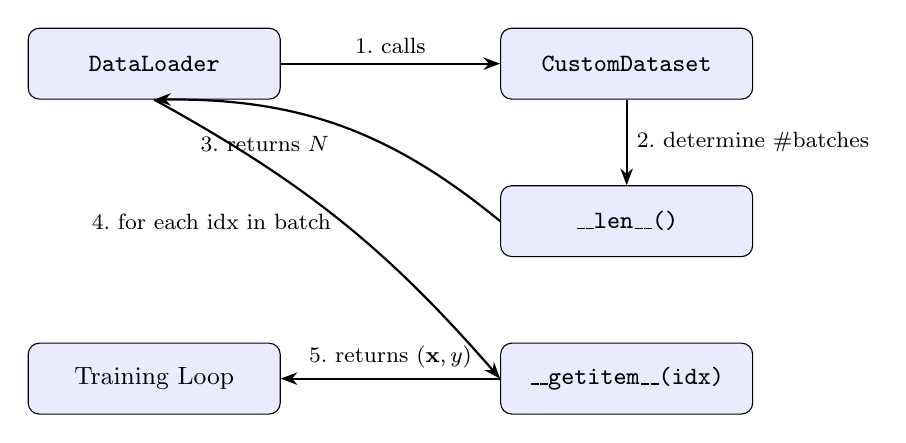
\begin{tikzpicture}[
  box/.style={rectangle, draw, rounded corners=4pt,
              minimum width=3.2cm, minimum height=0.9cm,
              fill=blue!8, font=\small},
  arrow/.style={-{Stealth[length=6pt]}, thick},
  note/.style={rectangle, draw=none, font=\footnotesize\itshape,
               text width=4cm, align=left}
]
  % Nodes
  \node[box] (dl)   at (0,0)    {\texttt{DataLoader}};
  \node[box] (ds)   at (6,0)    {\texttt{CustomDataset}};
  \node[box] (len)  at (6,-2)   {\texttt{\_\_len\_\_()}};
  \node[box] (gi)   at (6,-4)   {\texttt{\_\_getitem\_\_(idx)}};
  \node[box] (loop) at (0,-4)   {Training Loop};

  % Arrows
  \draw[arrow] (dl) -- node[above,font=\footnotesize]{1.\ calls} (ds);
  \draw[arrow] (ds) -- node[right,font=\footnotesize]{2.\ determine \#batches} (len);
  \draw[arrow] (len.west) to[bend right=20]
               node[below left,font=\footnotesize]{3.\ returns $N$} (dl.south);
  \draw[arrow] (dl.south) to[bend left=10]
               node[left,font=\footnotesize]{4.\ for each idx in batch} (gi.west);
  \draw[arrow] (gi) -- node[above,font=\footnotesize]{5.\ returns $(\mathbf{x},y)$} (loop);
\end{tikzpicture}
\caption{Call sequence between \texttt{DataLoader} and a custom \texttt{Dataset}.
The \texttt{DataLoader} first calls \texttt{\_\_len\_\_} to compute the number
of batches, then iteratively calls \texttt{\_\_getitem\_\_} to assemble each
batch tensor.}
\label{fig:dataset-dataloader}
\end{figure}

With $N = 4800$ and $B = 32$:
\begin{equation}
  \text{batches per epoch} = \left\lceil \frac{4800}{32} \right\rceil = 150
  \label{eq:batches}
\end{equation}

%% ============================================================
\section{Fashion-MNIST Dataset}
\label{sec:fashionmnist}
%% ============================================================

\subsection{Overview}
\label{subsec:fashionmnist-overview}

Fashion-MNIST is a dataset of grey-scale clothing images developed by Zalando
Research as a direct drop-in replacement for the classic handwritten-digit
MNIST dataset, but considerably more challenging.

\begin{table}[htbp]
  \centering
  \caption{Fashion-MNIST dataset properties}
  \label{tab:fashionmnist}
  \begin{tabular}{ll}
    \toprule
    \textbf{Property} & \textbf{Value} \\
    \midrule
    Image size          & $28 \times 28$ pixels \\
    Total pixels per image & $784$ \\
    Colour channels     & Grayscale (1 channel) \\
    Pixel value range   & 0 -- 255 (integer) \\
    Training samples    & 60{,}000 \\
    Test samples        & 10{,}000 \\
    Number of classes   & 10 \\
    Task type           & Multi-class classification \\
    Source              & Kaggle (\texttt{zalando-research/fashionmnist}) \\
    \bottomrule
  \end{tabular}
\end{table}

\subsection{Class Labels}
\label{subsec:class-labels}

Each image belongs to exactly one of the ten fashion categories listed in
\cref{tab:classes}.

\begin{table}[htbp]
  \centering
  \caption{Fashion-MNIST class labels}
  \label{tab:classes}
  \begin{tabular}{cl}
    \toprule
    \textbf{Label (integer)} & \textbf{Class name} \\
    \midrule
    0 & T-shirt / top \\
    1 & Trouser \\
    2 & Pullover \\
    3 & Dress \\
    4 & Coat \\
    5 & Sandal \\
    6 & Shirt \\
    7 & Sneaker \\
    8 & Bag \\
    9 & Ankle boot \\
    \bottomrule
  \end{tabular}
\end{table}

\subsection{ANN vs.\ CNN Representation}
\label{subsec:ann-vs-cnn}

The instructor explicitly highlights that this session uses the \emph{ANN
(fully connected)} approach, where each $28 \times 28$ image is
\emph{flattened} into a $784$-dimensional vector before being fed to the
network.  This loses spatial structure, which motivates the next topic:
Convolutional Neural Networks (CNNs), where the 2-D pixel grid is preserved.

\begin{keyinsight}[title=ANN vs.\ CNN on Image Data]
In an ANN for Fashion-MNIST:
\begin{itemize}
  \item The $28 \times 28$ image is flattened to a vector $\mathbf{x} \in \mathbb{R}^{784}$.
  \item All spatial relationships between neighbouring pixels are discarded.
  \item This is sufficient for simple benchmarks but sub-optimal for complex images.
\end{itemize}
CNNs (covered next) process the image as a 2-D grid, preserving local
spatial structure through convolutional filters.
\end{keyinsight}

\subsection{Data Preprocessing Pipeline}
\label{subsec:preprocessing}

The session uses a sample of 6{,}000 rows from the Kaggle \texttt{train.csv}
file (the full training set has 60{,}000 rows).  The preprocessing steps are:

\begin{enumerate}[label=\arabic*.]
  \item \textbf{Load CSV}: read 6{,}000 rows $\times$ 785 columns with
        \texttt{pandas.read\_csv}.  Column 0 is the label; columns
        1--784 are pixel values.
  \item \textbf{Split features and labels}: $\mathbf{X} = \text{df.iloc}[:,1:]$,
        $\mathbf{y} = \text{df.iloc}[:,0]$.
  \item \textbf{Train/test split}: 80\,\% train (4{,}800 rows),
        20\,\% test (1{,}200 rows) using \texttt{train\_test\_split}
        from scikit-learn.
  \item \textbf{Normalisation}: divide all pixel values by 255 so that
        $x_{ij} \in [0, 1]$.
  \item \textbf{Wrap in \texttt{CustomDataset}} and create
        \texttt{DataLoader} objects.
\end{enumerate}

The normalisation formula is:

\begin{equation}
  \tilde{x}_{ij} = \frac{x_{ij}}{255}, \quad x_{ij} \in \{0,\ldots,255\},
  \quad \tilde{x}_{ij} \in [0, 1]
  \label{eq:normalise}
\end{equation}

\begin{remark}
\label{rem:normalise}
Normalising pixel values to $[0,1]$ accelerates gradient-based optimisation
because features with large magnitudes produce large gradients, potentially
destabilising training.  Keeping all inputs in a common bounded range makes
the loss landscape better conditioned.
\end{remark}

%% ============================================================
\section{Neural Network Architecture}
\label{sec:architecture}
%% ============================================================

\subsection{Architecture Design}
\label{subsec:arch-design}

The target ANN for Fashion-MNIST classification has the following structure:

\begin{equation}
  784 \;\xrightarrow{\;\text{Linear}\;}\; 128
      \;\xrightarrow{\;\text{ReLU}\;}\;
      128 \;\xrightarrow{\;\text{Linear}\;}\; 64
      \;\xrightarrow{\;\text{ReLU}\;}\;
      64  \;\xrightarrow{\;\text{Linear}\;}\; 10
      \;\xrightarrow{\;\text{Softmax}\;}\; \hat{y}
  \label{eq:arch}
\end{equation}

Each layer performs a linear transformation followed by a non-linear
activation:

\begin{align}
  \mathbf{h}_1 &= \text{ReLU}(\mathbf{W}_1 \mathbf{x} + \mathbf{b}_1),
    \quad \mathbf{W}_1 \in \mathbb{R}^{128 \times 784},\;
          \mathbf{b}_1 \in \mathbb{R}^{128} \label{eq:layer1} \\
  \mathbf{h}_2 &= \text{ReLU}(\mathbf{W}_2 \mathbf{h}_1 + \mathbf{b}_2),
    \quad \mathbf{W}_2 \in \mathbb{R}^{64 \times 128},\;
          \mathbf{b}_2 \in \mathbb{R}^{64}  \label{eq:layer2} \\
  \mathbf{z}   &= \mathbf{W}_3 \mathbf{h}_2 + \mathbf{b}_3,
    \quad \mathbf{W}_3 \in \mathbb{R}^{10 \times 64},\;
          \mathbf{b}_3 \in \mathbb{R}^{10}   \label{eq:layer3} \\
  \hat{\mathbf{y}} &= \text{Softmax}(\mathbf{z}) \label{eq:softmax}
\end{align}

\subsection{TikZ Diagram of the ANN Architecture}
\label{subsec:arch-diagram}

\cref{fig:ann} shows the fully connected architecture.

\begin{figure}[htbp]
\centering
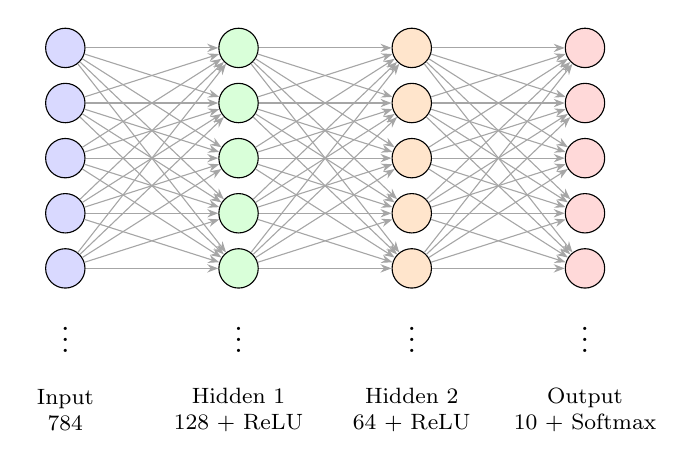
\begin{tikzpicture}[
  neuron/.style={circle, draw, fill=blue!15,
                 minimum size=0.5cm, inner sep=0pt},
  label_node/.style={rectangle, draw=none, font=\small\bfseries},
  arrow/.style={-{Stealth[length=4pt]}, gray!70, thin},
  layer_label/.style={font=\footnotesize, align=center}
]

% Column x-positions
\def\xIn{0}
\def\xH{2.2}
\def\xHH{4.4}
\def\xOut{6.6}

% Input layer (show 5 neurons + dots)
\foreach \i in {1,2,3,4,5}{
  \pgfmathsetmacro{\yy}{(\i-3)*0.7}
  \node[neuron] (I\i) at (\xIn,\yy) {};
}
\node[font=\large] at (\xIn,-2.2) {$\vdots$};

% Hidden layer 1 (show 5 neurons + dots)
\foreach \i in {1,2,3,4,5}{
  \pgfmathsetmacro{\yy}{(\i-3)*0.7}
  \node[neuron,fill=green!15] (H1\i) at (\xH,\yy) {};
}
\node[font=\large] at (\xH,-2.2) {$\vdots$};

% Hidden layer 2 (show 5 neurons + dots)
\foreach \i in {1,2,3,4,5}{
  \pgfmathsetmacro{\yy}{(\i-3)*0.7}
  \node[neuron,fill=orange!20] (H2\i) at (\xHH,\yy) {};
}
\node[font=\large] at (\xHH,-2.2) {$\vdots$};

% Output layer (show 5 neurons + dots)
\foreach \i in {1,2,3,4,5}{
  \pgfmathsetmacro{\yy}{(\i-3)*0.7}
  \node[neuron,fill=red!15] (O\i) at (\xOut,\yy) {};
}
\node[font=\large] at (\xOut,-2.2) {$\vdots$};

% Connections I->H1
\foreach \i in {1,2,3,4,5}{
  \foreach \j in {1,2,3,4,5}{
    \draw[arrow] (I\i) -- (H1\j);
  }
}

% Connections H1->H2
\foreach \i in {1,2,3,4,5}{
  \foreach \j in {1,2,3,4,5}{
    \draw[arrow] (H1\i) -- (H2\j);
  }
}

% Connections H2->O
\foreach \i in {1,2,3,4,5}{
  \foreach \j in {1,2,3,4,5}{
    \draw[arrow] (H2\i) -- (O\j);
  }
}

% Layer labels
\node[layer_label] at (\xIn,-3.2)  {Input\\784};
\node[layer_label] at (\xH,-3.2)   {Hidden 1\\128 + ReLU};
\node[layer_label] at (\xHH,-3.2)  {Hidden 2\\64 + ReLU};
\node[layer_label] at (\xOut,-3.2) {Output\\10 + Softmax};

\end{tikzpicture}
\caption{Fully connected ANN for Fashion-MNIST classification.
Inputs are the 784 normalised pixel values of a $28\times28$ greyscale image.
The two hidden layers use ReLU activation; Softmax is applied implicitly by
\texttt{nn.CrossEntropyLoss} during training.}
\label{fig:ann}
\end{figure}

\subsection{Activation Functions}
\label{subsec:activations}

\textbf{ReLU} (Rectified Linear Unit) is used in both hidden layers:
\begin{equation}
  \text{ReLU}(z) = \max(0, z)
  \label{eq:relu}
\end{equation}

\textbf{Softmax} converts raw output logits into a probability distribution
over the 10 classes:
\begin{equation}
  \text{Softmax}(z_k) = \frac{e^{z_k}}{\sum_{j=1}^{10} e^{z_j}},
  \quad k = 0, 1, \ldots, 9
  \label{eq:softmax-eq}
\end{equation}

\begin{remark}
\label{rem:softmax-in-loss}
In PyTorch, \texttt{nn.CrossEntropyLoss} combines the Softmax operation
with the negative log-likelihood loss.  Therefore it is \emph{not} necessary
(and is actually incorrect) to apply an explicit \texttt{nn.Softmax} layer
before the loss function.  The output of the final \texttt{nn.Linear} layer
(the raw logits $\mathbf{z}$) is passed directly to the loss.
\end{remark}

\subsection{Parameter Count}
\label{subsec:params}

The total number of learnable parameters is computed layer by layer.

\begin{table}[htbp]
  \centering
  \caption{Layer-wise parameter count for the $784 \to 128 \to 64 \to 10$ ANN}
  \label{tab:params}
  \begin{tabular}{lccr}
    \toprule
    \textbf{Layer} & \textbf{Input dim} & \textbf{Output dim} & \textbf{Parameters} \\
    \midrule
    Linear 1 (weights) & 784 & 128 & $784 \times 128 = 100{,}352$ \\
    Linear 1 (biases)  & --  & 128 & $128$ \\
    \textit{ReLU 1}    & 128 & 128 & $0$ \\
    Linear 2 (weights) & 128 & 64  & $128 \times 64 = 8{,}192$ \\
    Linear 2 (biases)  & --  & 64  & $64$ \\
    \textit{ReLU 2}    & 64  & 64  & $0$ \\
    Linear 3 (weights) & 64  & 10  & $64 \times 10 = 640$ \\
    Linear 3 (biases)  & --  & 10  & $10$ \\
    \midrule
    \textbf{Total} & & & \textbf{109,386} \\
    \bottomrule
  \end{tabular}
\end{table}

The dominant term is the first linear layer:
\begin{equation}
  \underbrace{784 \times 128}_{\text{weights}} + \underbrace{128}_{\text{biases}}
  = 100{,}480 \text{ parameters}
  \label{eq:first-layer-params}
\end{equation}

This accounts for $100{,}480 / 109{,}386 \approx 91.9\,\%$ of all learnable
parameters.

%% ============================================================
\section{nn.Module Implementation and Hands-On Walkthrough}
\label{sec:implementation}
%% ============================================================

\subsection{Toy nn.Module Example}
\label{subsec:toy-module}

Before building the full Fashion-MNIST model, the instructor demonstrates a
minimal \texttt{nn.Module} subclass to solidify the concept:

\begin{tcolorbox}[colback=gray!5!white, colframe=gray!60!black,
  fonttitle=\bfseries, title=Listing 3: Toy nn.Module (binary classification)]
\begin{verbatim}
import torch
import torch.nn as nn

class Model(nn.Module):
    def __init__(self, num_features):
        super().__init__()
        self.linear1  = nn.Linear(num_features, 3)
        self.relu     = nn.ReLU()
        self.linear2  = nn.Linear(3, 1)
        self.sigmoid  = nn.Sigmoid()

    def forward(self, features):
        out = self.linear1(features)
        out = self.relu(out)
        out = self.linear2(out)
        out = self.sigmoid(out)
        return out

# Usage
features = torch.rand(10, 5)          # 10 samples, 5 features
model    = Model(features.shape[1])   # num_features = 5
output   = model(features)            # calls forward()
# output shape: [10, 1]
\end{verbatim}
\end{tcolorbox}

\begin{example}[title=Two roles of nn.Module]
\begin{enumerate}[label=\arabic*.]
  \item \textbf{\texttt{\_\_init\_\_}}: Defines and registers all
        \emph{sub-modules} (layers). PyTorch tracks their parameters
        automatically for gradient computation.
  \item \textbf{\texttt{forward}}: Defines the computation graph,
        i.e.\ how data flows from input to output. Calling \texttt{model(x)}
        invokes \texttt{forward(x)} transparently.
\end{enumerate}
\end{example}

\subsection{MyNN: Full Fashion-MNIST Model}
\label{subsec:mynn}

The complete ANN used in the session is:

\begin{tcolorbox}[colback=gray!5!white, colframe=gray!60!black,
  fonttitle=\bfseries, title=Listing 4: MyNN -- Fashion-MNIST ANN]
\begin{verbatim}
class MyNN(nn.Module):
    def __init__(self, num_features):
        super().__init__()
        self.model = nn.Sequential(
            nn.Linear(num_features, 128),
            nn.ReLU(),
            nn.Linear(128, 64),
            nn.ReLU(),
            nn.Linear(64, 10)
            # No Softmax here: CrossEntropyLoss includes it
        )

    def forward(self, x):
        return self.model(x)
\end{verbatim}
\end{tcolorbox}

\subsection{nn.Sequential Container}
\label{subsec:sequential}

\texttt{nn.Sequential} chains modules in order.  The output of each module
automatically becomes the input of the next.  This models the mathematical
composition:

\begin{equation}
  f(\mathbf{x}) = \mathbf{W}_3 \cdot
    \text{ReLU}\!\left(\mathbf{W}_2 \cdot
      \text{ReLU}\!\left(\mathbf{W}_1 \mathbf{x} + \mathbf{b}_1\right)
      + \mathbf{b}_2\right)
    + \mathbf{b}_3
  \label{eq:sequential}
\end{equation}

\subsection{Loss Function and Optimiser}
\label{subsec:loss}

\begin{tcolorbox}[colback=gray!5!white, colframe=gray!60!black,
  fonttitle=\bfseries, title=Listing 5: Instantiating model, loss, and optimiser]
\begin{verbatim}
# Hyperparameters
num_epochs    = 100
learning_rate = 0.1

# Model
model     = MyNN(num_features=X_train.shape[1])

# Loss function (includes Softmax internally)
criterion = nn.CrossEntropyLoss()

# Optimiser: Stochastic Gradient Descent
optimizer = torch.optim.SGD(model.parameters(),
                            lr=learning_rate)
\end{verbatim}
\end{tcolorbox}

The cross-entropy loss for a single sample with true class $c$ and logit
vector $\mathbf{z}$ is:
\begin{equation}
  \mathcal{L}_{\text{CE}}(\mathbf{z}, c) =
  -\log\!\left(\frac{e^{z_c}}{\sum_{j=0}^{9} e^{z_j}}\right)
  = -z_c + \log\!\left(\sum_{j=0}^{9} e^{z_j}\right)
  \label{eq:ce-loss}
\end{equation}

\subsection{The Training Loop}
\label{subsec:training-loop}

\cref{alg:training} formalises the training procedure implemented in the
session notebook.

\begin{algorithm}[H]
\caption{Mini-Batch Training Loop for Fashion-MNIST ANN}
\label{alg:training}
\SetAlgoLined
\KwIn{train\_loader, model, criterion, optimizer, num\_epochs}
\KwOut{Trained model; epoch-level average loss printed each epoch}

\For{epoch $\leftarrow 1$ \KwTo \textup{num\_epochs}}{
  epoch\_loss $\leftarrow 0$ \;
  \For{(batch\_features, batch\_labels) \textbf{in} train\_loader}{
    \tcc{Step 1: Forward pass}
    outputs $\leftarrow$ model(batch\_features)\;
    \tcc{Step 2: Compute loss}
    loss $\leftarrow$ criterion(outputs, batch\_labels)\;
    \tcc{Step 3: Zero gradients, backward pass}
    optimizer.zero\_grad()\;
    loss.backward()\;
    \tcc{Step 4: Update parameters}
    optimizer.step()\;
    epoch\_loss $\leftarrow$ epoch\_loss $+$ loss.item()\;
  }
  avg\_loss $\leftarrow$ epoch\_loss $/ $ len(train\_loader)\;
  \textbf{print}(``Epoch'', epoch, ``Loss:'', avg\_loss)\;
}
\end{algorithm}

\begin{keyinsight}[title=The Four Steps of a Training Iteration]
Every mini-batch in every epoch executes exactly four operations:
\begin{enumerate}[label=\arabic*.]
  \item \textbf{Forward pass}: compute predictions $\hat{\mathbf{y}} = f(\mathbf{x}; \boldsymbol{\theta})$.
  \item \textbf{Loss computation}: evaluate $\mathcal{L}(\hat{\mathbf{y}}, \mathbf{y})$.
  \item \textbf{Backward pass}: compute $\nabla_{\boldsymbol{\theta}} \mathcal{L}$ via automatic differentiation.
  \item \textbf{Parameter update}: apply the SGD update rule (\cref{eq:sgd}).
\end{enumerate}
It is essential to call \texttt{optimizer.zero\_grad()} before
\texttt{loss.backward()} because PyTorch \emph{accumulates} gradients by
default across calls.
\end{keyinsight}

\subsection{Evaluation on the Test Set}
\label{subsec:evaluation}

After training, the model is switched to evaluation mode and accuracy is
computed:

\begin{tcolorbox}[colback=gray!5!white, colframe=gray!60!black,
  fonttitle=\bfseries, title=Listing 6: Test evaluation]
\begin{verbatim}
model.eval()
correct = 0
total   = 0

with torch.no_grad():
    for batch_features, batch_labels in test_loader:
        outputs    = model(batch_features)
        _, predicted = torch.max(outputs, dim=1)
        total   += batch_labels.size(0)
        correct += (predicted == batch_labels).sum().item()

accuracy = correct / total * 100
print(f"Test Accuracy: {accuracy:.2f}%")
\end{verbatim}
\end{tcolorbox}

The session reports a test accuracy of approximately \textbf{83\,\%} on the
1{,}200-sample test split (20\,\% of the 6{,}000-row sample dataset).

\begin{warningbox}[title=model.eval() is essential]
Calling \texttt{model.eval()} is not optional.  Certain layers (Dropout,
BatchNorm) behave differently during training versus inference.  Even if your
current architecture does not use these layers, it is best practice to always
set \texttt{model.eval()} before any inference or evaluation pass.  Pair it
with \texttt{torch.no\_grad()} to suppress gradient computation and reduce
memory usage.
\end{warningbox}

%% ============================================================
\section{torchinfo Model Summary}
\label{sec:torchinfo}
%% ============================================================

\subsection{Inspecting the Architecture with torchinfo}
\label{subsec:torchinfo}

The \texttt{torchinfo} library provides a Keras-style model summary for
PyTorch networks.  In the session:

\begin{tcolorbox}[colback=gray!5!white, colframe=gray!60!black,
  fonttitle=\bfseries, title=Listing 7: torchinfo summary call]
\begin{verbatim}
from torchinfo import summary
summary(model, input_size=(4800, 784))
\end{verbatim}
\end{tcolorbox}

The output (reproduced from the Colab notebook) is:

\begin{tcolorbox}[colback=black!5!white, colframe=black!40!white,
  fonttitle=\bfseries, title=torchinfo Output for MyNN]
\begin{verbatim}
=================================================================
Layer (type:depth-idx)    Output Shape        Param #
=================================================================
MyNN                      [4800, 10]          --
|-Sequential: 1-1         [4800, 10]          --
|  |-Linear: 2-1          [4800, 128]         100,480
|  |-ReLU: 2-2            [4800, 128]         --
|  |-Linear: 2-3          [4800, 64]          8,256
|  |-ReLU: 2-4            [4800, 64]          --
|  |-Linear: 2-5          [4800, 10]          650
=================================================================
Total params:             109,386
Trainable params:         109,386
Non-trainable params:     0
-----------------------------------------------------------------
Input size (MB):          15.05
Forward/backward size(MB):  7.76
Params size (MB):         0.44
=================================================================
\end{verbatim}
\end{tcolorbox}

\subsection{Verifying Parameter Counts}
\label{subsec:verify-params}

The \texttt{torchinfo} output can be verified analytically:

\begin{align}
  \text{Linear 1} &: 784 \times 128 + 128 = 100{,}480 \label{eq:p1} \\
  \text{Linear 2} &: 128 \times 64  + 64  = 8{,}256   \label{eq:p2} \\
  \text{Linear 3} &: 64  \times 10  + 10  = 650        \label{eq:p3} \\
  \text{Total}    &: 100{,}480 + 8{,}256 + 650 = 109{,}386 \label{eq:ptotal}
\end{align}

Note that \texttt{input\_size=(4800, 784)} specifies the full training set
shape for display purposes; the actual per-batch input shape during training
is $(32, 784)$.

%% ============================================================
\section{Complete Pipeline: Data Flow Diagram}
\label{sec:pipeline}
%% ============================================================

\cref{fig:pipeline} illustrates the complete end-to-end pipeline covered in
this session.

\begin{figure}[htbp]
\centering
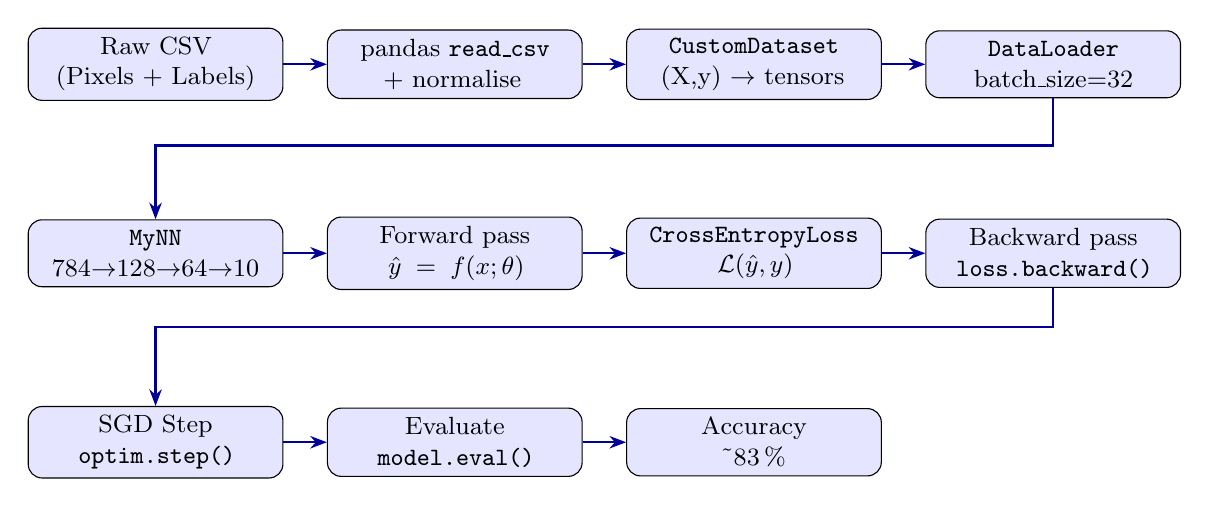
\begin{tikzpicture}[
  block/.style={rectangle, draw, rounded corners=5pt,
                fill=blue!10, minimum width=3.0cm,
                minimum height=0.85cm, font=\small,
                text centered, text width=3.0cm},
  decision/.style={diamond, draw, fill=yellow!15, font=\small,
                   text centered, aspect=2},
  arr/.style={-{Stealth[length=6pt]}, thick, blue!60!black},
  lab/.style={font=\footnotesize\itshape, midway}
]

\node[block] (raw)    at (0,0)     {Raw CSV\\(Pixels + Labels)};
\node[block] (pandas) at (3.8,0)   {pandas \texttt{read\_csv}\\+ normalise};
\node[block] (ds)     at (7.6,0)   {\texttt{CustomDataset}\\(X,y) $\to$ tensors};
\node[block] (dl)     at (11.4,0)  {\texttt{DataLoader}\\batch\_size=32};

\node[block] (model)  at (0,-2.4)  {\texttt{MyNN}\\$784{\to}128{\to}64{\to}10$};
\node[block] (fwd)    at (3.8,-2.4){Forward pass\\$\hat{y}=f(x;\theta)$};
\node[block] (loss)   at (7.6,-2.4){\texttt{CrossEntropyLoss}\\$\mathcal{L}(\hat{y},y)$};
\node[block] (bwd)    at (11.4,-2.4){Backward pass\\\texttt{loss.backward()}};

\node[block] (upd)    at (0,-4.8)  {SGD Step\\\texttt{optim.step()}};
\node[block] (eval)   at (3.8,-4.8){Evaluate\\\texttt{model.eval()}};
\node[block] (acc)    at (7.6,-4.8){Accuracy\\\textasciitilde83\,\%};

\draw[arr] (raw)    -- (pandas);
\draw[arr] (pandas) -- (ds);
\draw[arr] (ds)     -- (dl);
\draw[arr] (dl.south) -- ++(0,-0.6) -| (model.north);

\draw[arr] (model) -- (fwd);
\draw[arr] (fwd)   -- (loss);
\draw[arr] (loss)  -- (bwd);
\draw[arr] (bwd.south) -- ++(0,-0.5) -| (upd.north);

\draw[arr] (upd)  -- (eval);
\draw[arr] (eval) -- (acc);

\end{tikzpicture}
\caption{Complete end-to-end pipeline for Fashion-MNIST ANN training and
evaluation as implemented in Session~11.  The pipeline flows left to right,
then wraps to the next row.}
\label{fig:pipeline}
\end{figure}

%% ============================================================
\section{Q\&A Discussion Highlights}
\label{sec:qa}
%% ============================================================

Several important questions were raised during the session and are documented
here for completeness.

\subsection{Sigmoid vs.\ Softmax at the Output Layer}

\textbf{Question}: Do the neurons in this network use Sigmoid or Softmax?

\textbf{Answer}: Neither activation appears as an explicit \texttt{nn} module
in the model definition.  The hidden layers use ReLU.  The output layer
produces raw logits.  When \texttt{nn.CrossEntropyLoss} is called, it
internally applies Softmax and then computes the negative log-likelihood.  For
\emph{binary} classification, \texttt{nn.BCELoss} with a Sigmoid output would
be the appropriate choice.

The choice of output activation depends on the task type:
\begin{equation}
  \text{output activation} =
  \begin{cases}
    \text{Sigmoid} & \text{binary classification (2 classes)} \\
    \text{Softmax} & \text{multi-class classification ($>$2 classes)} \\
    \text{None (linear)} & \text{regression}
  \end{cases}
  \label{eq:activation-choice}
\end{equation}

\subsection{Streaming Data with DataLoader}

\textbf{Question}: Does PyTorch's \texttt{DataLoader} support streaming
(live) data feeds?

\textbf{Answer (instructor)}: The standard \texttt{DataLoader} is designed
for fixed-size datasets that can be indexed by integer position.  For
streaming scenarios (e.g.\ real-time sensor data), a custom iterable-style
\texttt{IterableDataset} subclass can be used, but this requires a different
implementation strategy.

\subsection{Gradient Zeroing -- Why Is It Necessary?}

\textbf{Question (implicit)}: Why is \texttt{optimizer.zero\_grad()} needed
before every backward pass?

\textbf{Answer}: PyTorch accumulates (adds) gradients to the
\texttt{.grad} attribute of each parameter tensor by default.  Without
zeroing, the gradient for batch $t$ would be the sum of all gradients from
batches $1, 2, \ldots, t$, which would corrupt the SGD update.

\begin{example}[title=Effect of not zeroing gradients]
Suppose the gradient of some weight $w$ is $+0.3$ in batch 1 and $-0.1$ in
batch 2.  Without zeroing, batch 2 would use $\nabla w = 0.3 + (-0.1) = +0.2$
instead of $-0.1$, giving an incorrect update direction.
\end{example}

\subsection{Building a Neural Network from Scratch}

\textbf{Question}: Is it possible to build a neural network without using
PyTorch?

\textbf{Answer}: Yes -- in the first weeks of the course the instructor
demonstrated manual implementation of forward propagation and gradient descent
using only NumPy, explicitly writing out $\mathbf{W}\mathbf{x} + \mathbf{b}$,
activation functions, and finite-difference gradient approximations.  PyTorch
automates the gradient computation (autograd), layer registration, and
optimisation steps that were done manually earlier.  The PyTorch abstraction
exists to make research and deployment tractable at scale.

%% ============================================================
\section{Summary and Conclusions}
\label{sec:summary}
%% ============================================================

\subsection{Key Concepts Covered}

Session~11 delivered a complete hands-on implementation cycle covering:

\begin{enumerate}[label=\arabic*.]
  \item \textbf{Dataset abstraction}: \texttt{CustomDataset(Dataset)} with
        \texttt{\_\_init\_\_}, \texttt{\_\_len\_\_}, and
        \texttt{\_\_getitem\_\_}.  The constructor converts raw arrays to
        typed tensors automatically on object creation.

  \item \textbf{DataLoader}: batches the dataset into mini-batches of size
        32 with shuffling for training data (to prevent class-sequential
        batches) and without shuffling for test data (for reproducibility).

  \item \textbf{Fashion-MNIST}: a benchmark of 70{,}000 $28\times28$
        greyscale clothing images across 10 classes; pixel values normalised
        to $[0,1]$.

  \item \textbf{ANN architecture} $784 \to 128 \to 64 \to 10$ with ReLU
        hidden activations and implicit Softmax via
        \texttt{nn.CrossEntropyLoss}; total 109{,}386 trainable parameters.

  \item \textbf{Training loop}: four-step mini-batch procedure (forward,
        loss, backward, update) repeated for 100 epochs $\times$ 150
        batches = 15{,}000 weight updates.

  \item \textbf{Evaluation}: test accuracy of $\approx 83\,\%$ on a
        1{,}200-sample hold-out set after training on 4{,}800 samples.

  \item \textbf{torchinfo}: layer-wise model inspection tool confirming
        output shapes and parameter counts.
\end{enumerate}

\subsection{What Comes Next}

The session closes with a preview of upcoming topics:

\begin{itemize}
  \item \textbf{CNN} (Convolutional Neural Network): the same Fashion-MNIST
        dataset will be revisited using convolutional layers that preserve
        the 2-D spatial structure of the image rather than flattening it.
  \item \textbf{Dropout and Batch Normalisation}: the significance of
        \texttt{model.eval()} vs.\ \texttt{model.train()} will be explored
        in detail when these regularisation layers are introduced.
  \item \textbf{Larger datasets}: using \texttt{torchvision.datasets} to
        load the full 60{,}000-sample version of Fashion-MNIST directly
        without downloading a CSV from Kaggle.
\end{itemize}

\subsection{Comparison: ANN vs.\ CNN for Image Classification}

\begin{table}[htbp]
  \centering
  \caption{Comparison of ANN and CNN approaches for Fashion-MNIST}
  \label{tab:ann-vs-cnn}
  \begin{tabularx}{\linewidth}{lXX}
    \toprule
    \textbf{Aspect} & \textbf{ANN (Session 11)} & \textbf{CNN (upcoming)} \\
    \midrule
    Input format & Flattened vector $\mathbb{R}^{784}$ &
      2-D grid $\mathbb{R}^{1 \times 28 \times 28}$ \\
    Spatial structure & Discarded & Preserved via conv.\ filters \\
    Parameters & 109{,}386 (dense) &
      Fewer (shared filter weights) \\
    Typical accuracy & $\approx 83\text{--}87\,\%$ &
      $\approx 90\text{--}94\,\%$ \\
    Key layers & \texttt{nn.Linear}, \texttt{nn.ReLU} &
      \texttt{nn.Conv2d}, \texttt{nn.MaxPool2d}, \texttt{nn.Linear} \\
    \bottomrule
  \end{tabularx}
\end{table}

\begin{keyinsight}[title=Core Takeaway]
The Dataset--DataLoader--Model--TrainingLoop pattern introduced in this
session is \emph{universal}.  Regardless of whether the model is an ANN, CNN,
RNN, or Transformer, the same four-step training loop and the same
Dataset/DataLoader infrastructure apply.  Mastering this pattern is the
foundation for all subsequent deep learning work in PyTorch.
\end{keyinsight}

\clearpage

%% ============================================================
%% Session 12: ANN Regularisation and CNN Introduction
%% ============================================================
\part{Session 12: ANN Regularisation and CNN Introduction}

% ============================================================

%% ---- Title page ----
\begin{titlepage}
  \centering
  \vspace*{2cm}
  {\LARGE\bfseries Deep Learning Course\\[0.4em]
   \rule{\linewidth}{0.5pt}\\[0.6em]
   Session 12 Lecture Notes}\\[1.2em]
  {\large\itshape ANN Regularisation (BatchNorm, Dropout, $\Ltwo$)\\
   on Fashion-MNIST and Introduction to CNNs}\\[2em]
  \begin{tabular}{ll}
    \textbf{Session:}     & 12 of 24 \\[0.3em]
    \textbf{Topic:}       & ANN Optimisation + CNN Foundations \\[0.3em]
    \textbf{Instructors:} & Prof.\ S R M Prasanna \&\ Dr.\ Sunil Saumya \\[0.3em]
    \textbf{Institute:}   & IIIT Dharwad (IIITDwd) \\[0.3em]
    \textbf{Slide Decks:} & \texttt{04-PyTorchDL-NNmodule} (ANN),
                            \texttt{03-DL-CNN} (CNN) \\[0.3em]
    \textbf{Duration:}    & $\approx 1$\,hr\,32\,min \\[0.3em]
    \textbf{Date:}        & December 26, 2025 \\
  \end{tabular}\\[3em]
  \begin{abstract}
    \noindent
    Session 12 bridges the hands-on ANN experiments from Session 11 with the
    theoretical and practical foundations of Convolutional Neural Networks
    (CNNs).  The first hour is devoted to reviewing the three versions of the
    Fashion-MNIST ANN built in the previous session, identifying the
    overfitting gap (training accuracy 98\,\% vs.\ test accuracy 88\,\%),
    and introducing three complementary regularisation strategies:
    $\Ltwo$~weight-decay, Batch Normalisation, and Dropout.  An optimised
    fourth version combines all three remedies and achieves a tighter
    train/test gap ($93\,\% / 88\,\%$).  The second half of the session is
    presented by Prof.\ Prasanna, who motivates CNNs from first principles
    --- the spatial structure of image data, the history of the ImageNet
    challenge, and the fundamental distinction between matrix multiplication
    (used in ANNs) and the convolution operation (used in CNNs).
  \end{abstract}
  \vfill
  {\small These notes were compiled from the video transcript and visual
   extractions of the session recording.}
\end{titlepage}

%% ---- Table of Contents ----

\newpage

% ============================================================
\section{Introduction and Session Overview}
\label{sec:intro}
% ============================================================

Session 12 occupies a pivotal position in the course: it closes the ANN
regularisation arc that began in Session 11 and opens the new chapter on
Convolutional Neural Networks.  The session is co-taught:
Dr.\ Sunil Saumya leads the first $\approx$50 minutes, covering regularisation
theory and the Google Colab notebook, while Prof.\ S R M Prasanna presents the
CNN motivation and introduction from $\approx$51 minutes onwards.

\subsection{Learning Objectives}
\label{sec:intro:objectives}

By the end of this session, students should be able to:

\begin{enumerate}[label=\textbf{O\arabic*.}]
  \item Explain the concept of overfitting and diagnose it from the
        train/test accuracy gap.
  \item Apply $\Ltwo$ regularisation (weight decay) via the
        \texttt{weight\_decay} parameter of PyTorch optimisers.
  \item Insert \texttt{nn.BatchNorm1d} and \texttt{nn.Dropout} layers into an
        \texttt{nn.Sequential} model in the correct order.
  \item Describe the intuition behind dropout as an implicit ensemble of
        sub-networks.
  \item State the key differences between a fully-connected ANN layer (matrix
        multiplication) and a CNN layer (convolution with a kernel).
  \item Define the terms \emph{kernel}, \emph{filter}, and \emph{feature map}
        in the CNN context.
\end{enumerate}

\subsection{Session Roadmap}
\label{sec:intro:roadmap}

The session proceeds in three logical stages:

\begin{enumerate}
  \item \textbf{Recap} (0:00--0:25): Dr.\ Saumya reviews the three ANN
        versions built on Fashion-MNIST in the previous session, identifies
        the overfitting problem, and lists the remedies to be explored today.
  \item \textbf{ANN Regularisation} (0:25--0:50): Live coding in Google Colab
        demonstrating BatchNorm, Dropout, and $\Ltwo$ weight-decay,
        followed by a student Q\&A session.
  \item \textbf{CNN Introduction} (0:51--1:33): Prof.\ Prasanna introduces
        the historical motivation for CNNs, the concept of spatial
        data structure, and the convolution operation.
\end{enumerate}

% ============================================================
\section{Background and Prerequisites}
\label{sec:background}
% ============================================================

\subsection{The Fashion-MNIST Dataset}
\label{sec:background:fashionmnist}

Fashion-MNIST \cite{xiao2017fashionmnist} is a drop-in replacement for the
classic MNIST handwritten-digits dataset.  It contains $70{,}000$ grayscale
images ($28\times28$ pixels each) belonging to 10 clothing categories
(T-shirt, Trouser, Pullover, \ldots, Ankle boot).  The standard split
provides $60{,}000$ training samples and $10{,}000$ test samples.

\begin{keyinsight}
  Each $28\times28$ image is \emph{flattened} into a 784-dimensional vector
  before being fed into an ANN.  This discards all spatial (2D) structure ---
  the primary motivation for CNNs introduced in \cref{sec:cnn_intro}.
\end{keyinsight}

\subsection{PyTorch Data Pipeline Recap}
\label{sec:background:pipeline}

Two PyTorch classes handle data loading:

\begin{itemize}
  \item \textbf{\texttt{Dataset}}: Loads raw data and converts it to
        \texttt{torch.float32} tensors (features) and \texttt{torch.long}
        tensors (labels).  Implements \texttt{\_\_init\_\_},
        \texttt{\_\_len\_\_}, and \texttt{\_\_getitem\_\_}.
  \item \textbf{\texttt{DataLoader}}: Wraps a \texttt{Dataset} and provides
        shuffled mini-batches via the inner loop.  The \texttt{batch\_size}
        parameter controls how many samples are drawn at once.
\end{itemize}

The relationship can be summarised as:

\[
  \underbrace{\texttt{DataLoader}}_{\text{mini-batch generator}}
  \xrightarrow{\text{calls}}
  \underbrace{\texttt{Dataset.\_\_getitem\_\_}(i)}_{\text{returns one sample}}
\]

\subsection{The Training Loop}
\label{sec:background:loop}

Every mini-batch passes through four canonical steps:

\begin{enumerate}
  \item \textbf{Forward pass}: compute predictions $\hat{y} = f_\theta(x)$.
  \item \textbf{Loss}: compute $\mathcal{L}(\hat{y}, y)$.
  \item \textbf{Backward pass}: compute gradients via
        \texttt{loss.backward()}.
  \item \textbf{Weight update}: apply \texttt{optimizer.step()}.
\end{enumerate}

% ============================================================
\section{ANN Architecture for Fashion-MNIST}
\label{sec:ann_arch}
% ============================================================

\subsection{Baseline Architecture}
\label{sec:ann_arch:baseline}

The baseline network maps the flattened input ($784$ features) through two
hidden layers to a 10-class softmax output:

\begin{equation}
  \label{eq:ann_dims}
  784 \;\xrightarrow{\text{Linear}+\text{ReLU}}\; 128
      \;\xrightarrow{\text{Linear}+\text{ReLU}}\; 64
      \;\xrightarrow{\text{Linear}}\; 10
\end{equation}

\Cref{fig:ann_arch} shows the architecture diagram as presented on the
lecture slide.

\begin{figure}[htbp]
  \centering
  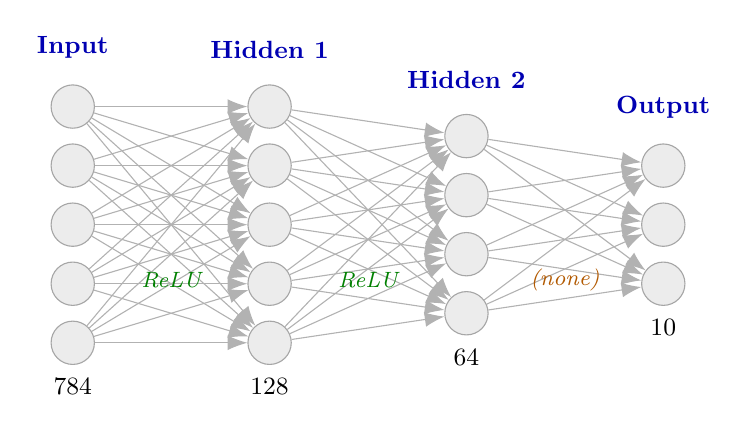
\begin{tikzpicture}[
      node distance=2.2cm,
      neuron/.style={circle, draw=gray!70, fill=gray!15,
                     minimum size=0.55cm, inner sep=0pt},
      layer/.style={rectangle, draw=blue!40, fill=blue!5,
                    rounded corners=3pt, minimum width=1.1cm,
                    minimum height=4.5cm},
      lbl/.style={font=\small\bfseries, text=blue!70!black},
      arr/.style={-{Latex[length=2.5mm]}, gray!60, line width=0.4pt}
    ]
    %% Input layer
    \foreach \i in {1,...,5}{
      \node[neuron] (I\i) at (0, {-(\i-1)*0.75}) {};
    }
    \node[lbl, above=0.2cm of I1] {Input};
    \node[font=\small, below=0.05cm of I5] {$784$};

    %% Hidden layer 1
    \foreach \i in {1,...,5}{
      \node[neuron] (H1\i) at (2.5, {-(\i-1)*0.75}) {};
    }
    \node[lbl, above=0.2cm of H11] {Hidden 1};
    \node[font=\small, below=0.05cm of H15] {$128$};

    %% Hidden layer 2
    \foreach \i in {1,...,4}{
      \node[neuron] (H2\i) at (5.0, {-(\i-1)*0.75 - 0.375}) {};
    }
    \node[lbl, above=0.2cm of H21] {Hidden 2};
    \node[font=\small, below=0.05cm of H24] {$64$};

    %% Output layer
    \foreach \i in {1,...,3}{
      \node[neuron] (O\i) at (7.5, {-(\i-1)*0.75 - 0.75}) {};
    }
    \node[lbl, above=0.2cm of O1] {Output};
    \node[font=\small, below=0.05cm of O3] {$10$};

    %% Connections I -> H1
    \foreach \i in {1,...,5}{
      \foreach \j in {1,...,5}{
        \draw[arr] (I\i) -- (H1\j);
      }
    }
    %% Connections H1 -> H2
    \foreach \i in {1,...,5}{
      \foreach \j in {1,...,4}{
        \draw[arr] (H1\i) -- (H2\j);
      }
    }
    %% Connections H2 -> O
    \foreach \i in {1,...,4}{
      \foreach \j in {1,...,3}{
        \draw[arr] (H2\i) -- (O\j);
      }
    }

    %% Activation labels
    \node[font=\footnotesize\itshape, text=green!50!black]
      at (1.25, -2.2) {ReLU};
    \node[font=\footnotesize\itshape, text=green!50!black]
      at (3.75, -2.2) {ReLU};
    \node[font=\footnotesize\itshape, text=orange!70!black]
      at (6.25, -2.2) {(none)};
  \end{tikzpicture}
  \caption{ANN architecture for Fashion-MNIST: $784\to128\to64\to10$.
           Connections are fully connected between consecutive layers.
           (Only a representative subset of neurons is drawn.)}
  \label{fig:ann_arch}
\end{figure}

\subsection{PyTorch Implementation}
\label{sec:ann_arch:impl}

The baseline model is implemented using \texttt{nn.Sequential}:

\begin{example}[title=Baseline ANN (Version 1 -- CPU, 6{,}000 samples)]
\begin{verbatim}
class MyANN(nn.Module):
    def __init__(self, num_features):
        super().__init__()
        self.model = nn.Sequential(
            nn.Linear(num_features, 128),
            nn.ReLU(),
            nn.Linear(128, 64),
            nn.ReLU(),
            nn.Linear(64, 10)
        )

    def forward(self, x):
        return self.model(x)

learning_rate = 0.1
epochs        = 100
\end{verbatim}
\end{example}

\subsection{Version 2: Full Dataset on GPU}
\label{sec:ann_arch:gpu}

In Version 2, the full 60{,}000-sample training set is used and the model
and data are moved to the GPU:

\begin{verbatim}
device = "cuda" if torch.cuda.is_available() else "cpu"
model  = MyANN(X_train.shape[1]).to(device)

# Inside the training loop:
X_batch = X_batch.to(device)
y_batch = y_batch.to(device)
\end{verbatim}

\begin{table}[htbp]
  \centering
  \caption{Performance comparison across ANN versions on Fashion-MNIST.}
  \label{tab:ann_versions}
  \begin{tabular}{clcccc}
    \toprule
    \textbf{Version} & \textbf{Description}
      & \textbf{Data} & \textbf{Train Acc.}
      & \textbf{Test Acc.} & \textbf{Overfit Gap} \\
    \midrule
    V1 & Baseline, CPU          & 6{,}000  & --    & 83\,\% & -- \\
    V2 & Full data, GPU         & 60{,}000 & 98\,\% & 88\,\% & 10\,\% \\
    V3 & BatchNorm + Dropout + $\Ltwo$ & 60{,}000 & 93\,\% & 88\,\% & 5\,\% \\
    \bottomrule
  \end{tabular}
\end{table}

\cref{tab:ann_versions} summarises the progression.  Moving from Version 2
to Version 3 reduces the training accuracy from 98\,\% to 93\,\% while
holding test accuracy constant at 88\,\%, demonstrating that the overfit
gap has been halved.

% ============================================================
\section{Overfitting and Regularisation Techniques}
\label{sec:regularisation}
% ============================================================

\subsection{Diagnosing Overfitting}
\label{sec:regularisation:diagnosis}

\begin{definition}[Overfitting]
  \label{def:overfitting}
  A model is said to \emph{overfit} the training data when it achieves
  significantly higher accuracy (or lower loss) on the training set than on
  an unseen test set.  Formally, if $\text{acc}_{\text{train}} \gg
  \text{acc}_{\text{test}}$, the model has learned spurious patterns
  (memorised the data) rather than generalising.
\end{definition}

In the session, this was observed as:

\begin{align}
  \text{Training accuracy} &= 98\,\% \notag \\
  \text{Test accuracy}     &= 88\,\% \notag \\
  \text{Gap}               &= 10\,\% \quad \Longrightarrow \quad \text{overfitting}
  \label{eq:overfit_gap}
\end{align}

\begin{keyinsight}
  The goal of regularisation is \emph{not} necessarily to improve test
  accuracy, but to \emph{reduce the gap} between train and test accuracy,
  thereby producing a model that generalises better.
\end{keyinsight}

\subsection{Strategies to Combat Overfitting}
\label{sec:regularisation:strategies}

The instructor outlined four strategies, in order of practicality for this
experiment:

\begin{enumerate}[label=\textbf{S\arabic*.}]
  \item \textbf{Add more data} --- increases diversity seen during training;
        not available here (60{,}000 is the full dataset).
  \item \textbf{Reduce model complexity} --- fewer hidden units or layers;
        the 2-layer network is already modest, so this has limited effect.
  \item \textbf{Early stopping} --- monitor validation accuracy and halt
        training when it plateaus.
  \item \textbf{Explicit regularisation} --- Dropout, Batch Normalisation,
        and $\Ltwo$ penalty (weight decay); the focus of this session.
\end{enumerate}

\subsection{\texorpdfstring{$\Ltwo$}{L2} Regularisation (Weight Decay)}
\label{sec:regularisation:l2}

\subsubsection{Concept}
\label{sec:regularisation:l2:concept}

$\Ltwo$ regularisation adds a penalty proportional to the squared magnitude
of all weights to the loss function:

\begin{equation}
  \label{eq:l2_loss}
  \mathcal{L}_{\text{total}}
    = \mathcal{L}_{\text{data}}
    + \lambda \sum_{i} w_i^2
\end{equation}

where $\lambda > 0$ is the regularisation strength (hyper-parameter) and
$w_i$ denotes the $i$-th learnable weight.

\begin{keyinsight}
  The gradient of the $\Ltwo$ penalty with respect to $w_i$ is $2\lambda
  w_i$.  When added to the ordinary gradient, this \emph{shrinks} every
  weight at each update step, which is why the technique is also known as
  \textbf{weight decay}.
\end{keyinsight}

\subsubsection{Effect on Gradient Descent}
\label{sec:regularisation:l2:grad}

Let $\eta$ be the learning rate.  The weight update rule becomes:

\begin{align}
  \label{eq:l2_update}
  w_i^{(t+1)}
    &= w_i^{(t)} - \eta \frac{\partial \mathcal{L}_{\text{data}}}{\partial w_i}
       - \eta \cdot 2\lambda w_i^{(t)} \notag \\
    &= w_i^{(t)}\bigl(1 - 2\eta\lambda\bigr)
       - \eta \frac{\partial \mathcal{L}_{\text{data}}}{\partial w_i}
\end{align}

The factor $(1 - 2\eta\lambda)$ is less than 1, so the weight is
multiplicatively decayed at each step, preventing any single weight from
growing excessively large.

\subsubsection{PyTorch Implementation}
\label{sec:regularisation:l2:code}

In PyTorch, $\Ltwo$ regularisation is passed directly to the optimiser via
the \texttt{weight\_decay} parameter (equivalent to $\lambda$):

\begin{verbatim}
optimizer = torch.optim.Adam(
    model.parameters(),
    lr=0.01,
    weight_decay=1e-4   # lambda = 0.0001
)
\end{verbatim}

\begin{warningbox}
  Setting \texttt{weight\_decay} too high forces all weights toward zero,
  causing \emph{underfitting}.  Conversely, too small a value provides
  negligible regularisation.  The instructor recommended $\lambda \approx
  10^{-4}$ as a safe starting point.
\end{warningbox}

\subsection{Batch Normalisation}
\label{sec:regularisation:batchnorm}

\subsubsection{Motivation}
\label{sec:regularisation:batchnorm:motivation}

During training, the distribution of activations feeding into each layer
shifts as earlier weights are updated --- a phenomenon known as
\emph{internal covariate shift}.  This forces downstream layers to
continually adapt, slowing convergence.

\subsubsection{Mathematical Formulation}
\label{sec:regularisation:batchnorm:math}

For a mini-batch $\mathcal{B} = \{z_1, \ldots, z_m\}$ of pre-activation
values at one layer, Batch Normalisation \cite{ioffe2015batchnorm} computes:

\begin{align}
  \label{eq:batchnorm}
  \mu_\mathcal{B} &= \frac{1}{m}\sum_{i=1}^{m} z_i
    & &\text{(batch mean)} \notag \\
  \sigma^2_\mathcal{B} &= \frac{1}{m}\sum_{i=1}^{m}(z_i - \mu_\mathcal{B})^2
    & &\text{(batch variance)} \notag \\
  \hat{z}_i &= \frac{z_i - \mu_\mathcal{B}}
                    {\sqrt{\sigma^2_\mathcal{B} + \epsilon}}
    & &\text{(normalise)} \\
  y_i &= \gamma \hat{z}_i + \beta
    & &\text{(scale and shift)} \notag
\end{align}

where $\gamma$ (scale) and $\beta$ (shift) are \emph{learnable parameters}
and $\epsilon$ is a small constant for numerical stability.

\subsubsection{Placement in the Layer Stack}
\label{sec:regularisation:batchnorm:placement}

The usual practice, as demonstrated in the session, is:

\[
  \texttt{Linear} \;\longrightarrow\;
  \texttt{BatchNorm1d} \;\longrightarrow\;
  \texttt{ReLU} \;\longrightarrow\;
  \texttt{Dropout}
\]

Batch Normalisation is applied \emph{before} the activation so that the
activation function (e.g.\ ReLU, sigmoid) receives values in a well-bounded
range, preventing saturation.

\subsection{Dropout}
\label{sec:regularisation:dropout}

\subsubsection{Concept}
\label{sec:regularisation:dropout:concept}

Dropout \cite{srivastava2014dropout} randomly deactivates a fraction $p$ of
neurons in a layer during each forward pass of training.

\begin{definition}[Dropout Mask]
  \label{def:dropout_mask}
  Let $\mathbf{h} \in \mathbb{R}^n$ be the post-activation vector for a
  layer of $n$ neurons.  The dropout mask $\mathbf{m} \in \{0,1\}^n$ is
  drawn independently for each element:
  \[
    m_i \sim \mathrm{Bernoulli}(1-p)
  \]
  The masked output is $\tilde{\mathbf{h}} = \mathbf{m} \odot \mathbf{h}$,
  where $\odot$ denotes element-wise multiplication.  At inference, no
  masking is applied and activations are scaled by $(1-p)$ to preserve
  expected magnitude.
\end{definition}

\subsubsection{Intuition: Implicit Ensemble}
\label{sec:regularisation:dropout:intuition}

The instructor drew an analogy with \emph{Random Forests}:

\begin{keyinsight}
  With $n$ neurons and dropout probability $p$, there are $2^n$ possible
  sub-networks.  Each mini-batch effectively trains a \emph{different}
  sub-network.  The final model can be thought of as an implicit
  \textbf{ensemble} of exponentially many networks that share weights.
  Because each sub-network sees a different architecture, co-adaptation of
  neurons is prevented and the model is forced to learn \emph{redundant}
  representations --- a powerful regulariser.
\end{keyinsight}

\subsubsection{Training vs.\ Inference Behaviour}
\label{sec:regularisation:dropout:train_vs_test}

A crucial point raised by students in the session Q\&A:

\begin{table}[htbp]
  \centering
  \caption{Dropout behaviour during training vs.\ inference.}
  \label{tab:dropout_mode}
  \begin{tabular}{lcc}
    \toprule
    \textbf{Phase} & \textbf{Masking Applied?} & \textbf{PyTorch call} \\
    \midrule
    Training   & Yes (random $p$-fraction zeroed) & \texttt{model.train()} \\
    Inference  & No (all neurons active, scaled)  & \texttt{model.eval()}  \\
    \bottomrule
  \end{tabular}
\end{table}

\subsubsection{Dropout Hyperparameter}
\label{sec:regularisation:dropout:hyperparam}

The parameter $p$ (fraction of neurons dropped) controls the trade-off:

\begin{itemize}
  \item Typical range: $p \in [0.2,\, 0.5]$.
  \item Higher $p$ ($\approx 0.4$--$0.5$): stronger regularisation, useful
        when severe overfitting is detected.
  \item Lower $p$ ($\approx 0.1$--$0.2$): milder regularisation, appropriate
        when the model underfits or has few parameters.
\end{itemize}

In the session notebook, $p = 0.3$ was used, dropping 30\,\% of neurons
in each hidden layer.

\subsection{Optimised ANN (Version 3)}
\label{sec:regularisation:v3}

\begin{example}[title=Optimised ANN (Version 3 -- BatchNorm + Dropout + $\Ltwo$)]
\begin{verbatim}
class MyANN(nn.Module):
    def __init__(self, num_features):
        super().__init__()
        self.model = nn.Sequential(
            nn.Linear(num_features, 128),
            nn.BatchNorm1d(128),      # normalise before activation
            nn.ReLU(),
            nn.Dropout(p=0.3),        # drop 30% after activation
            nn.Linear(128, 64),
            nn.BatchNorm1d(64),
            nn.ReLU(),
            nn.Dropout(p=0.3),
            nn.Linear(64, 10)
        )

    def forward(self, x):
        return self.model(x)

learning_rate = 0.01
epochs        = 100
model = MyANN(X_train.shape[1]).to(device)
optimizer = torch.optim.Adam(model.parameters(),
                             lr=learning_rate,
                             weight_decay=1e-4)

train_loader = DataLoader(train_dataset, batch_size=32,
                          shuffle=True, pin_memory=True)
test_loader  = DataLoader(test_dataset,  batch_size=32,
                          shuffle=False, pin_memory=True)
\end{verbatim}
\end{example}

\cref{fig:layer_stack} illustrates the layer ordering inside one block of
the optimised model.

\begin{figure}[htbp]
  \centering
  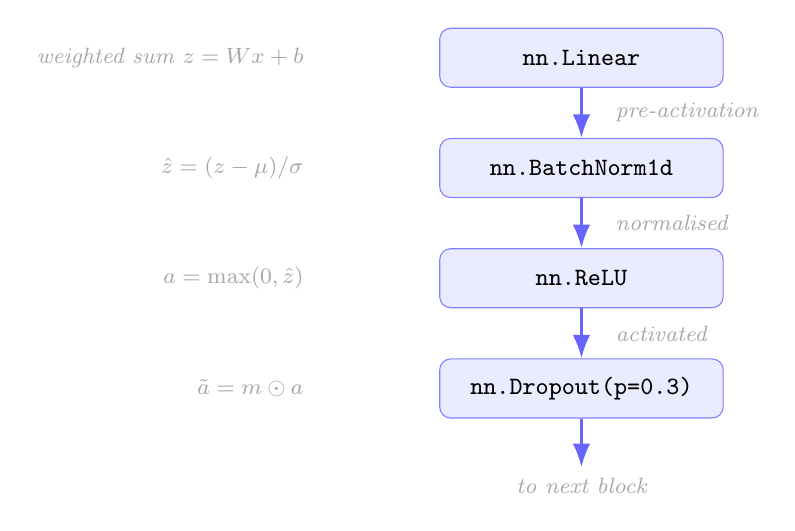
\begin{tikzpicture}[
      box/.style={rectangle, draw=blue!50, fill=blue!8,
                  rounded corners=4pt, minimum width=3.6cm,
                  minimum height=0.75cm, align=center,
                  font=\small},
      arr/.style={-{Latex[length=3mm]}, blue!60, line width=1pt},
      lbl/.style={font=\footnotesize\itshape, text=gray!70}
    ]
    \node[box] (L)  at (0,0)    {\texttt{nn.Linear}};
    \node[box] (BN) at (0,-1.4) {\texttt{nn.BatchNorm1d}};
    \node[box] (R)  at (0,-2.8) {\texttt{nn.ReLU}};
    \node[box] (D)  at (0,-4.2) {\texttt{nn.Dropout(p=0.3)}};

    \draw[arr] (L)  -- (BN)
      node[midway, right=3mm, lbl] {pre-activation};
    \draw[arr] (BN) -- (R)
      node[midway, right=3mm, lbl] {normalised};
    \draw[arr] (R)  -- (D)
      node[midway, right=3mm, lbl] {activated};
    \draw[arr] (D)  -- +(0,-1.0)
      node[below, lbl] {to next block};

    \node[lbl, left=1.6cm of L]  {weighted sum $z = Wx+b$};
    \node[lbl, left=1.6cm of BN] {$\hat{z} = (z-\mu)/\sigma$};
    \node[lbl, left=1.6cm of R]  {$a = \max(0,\hat{z})$};
    \node[lbl, left=1.6cm of D]  {$\tilde{a} = m \odot a$};
  \end{tikzpicture}
  \caption{Layer ordering within a single regularised block of the Version 3
           ANN.  BatchNorm is applied before the activation to ensure inputs
           are in a well-bounded range; Dropout is applied after the
           activation so that complete neuron outputs are masked.}
  \label{fig:layer_stack}
\end{figure}

% ============================================================
\section{Training Algorithm}
\label{sec:algorithm}
% ============================================================

\begin{algorithm}[H]
  \caption{Mini-Batch Training with BatchNorm, Dropout, and $\Ltwo$}
  \label{alg:training}
  \SetAlgoLined
  \KwIn{Training set $\mathcal{D}_{\text{train}}$,
        test set $\mathcal{D}_{\text{test}}$,
        model $f_\theta$ with BatchNorm and Dropout layers,
        learning rate $\eta$, weight decay $\lambda$,
        dropout probability $p$, epochs $E$, batch size $B$}
  \KwOut{Trained parameters $\theta^*$}

  Initialise $\theta$ (Xavier / He initialisation)\;
  Set \texttt{device} $\leftarrow$ \texttt{cuda} if GPU available else \texttt{cpu}\;
  Move $f_\theta$ and data to \texttt{device}\;
  Create \texttt{optimizer} $\leftarrow$ Adam($\theta$, lr=$\eta$, weight\_decay=$\lambda$)\;
  Create \texttt{train\_loader} with shuffle=True, batch\_size=$B$\;

  \For{epoch $= 1$ \KwTo $E$}{
    $f_\theta$.\texttt{train}()\tcp*{Enable BatchNorm statistics; enable Dropout}
    total\_loss $\leftarrow 0$\;

    \ForEach{$(X_b, y_b)$ in \texttt{train\_loader}}{
      $X_b, y_b \leftarrow X_b$.\texttt{to(device)}, $y_b$.\texttt{to(device)}\;
      \texttt{optimizer.zero\_grad()}\;
      $\hat{y}_b \leftarrow f_\theta(X_b)$\tcp*{Forward pass (Dropout active)}
      $\ell \leftarrow$ CrossEntropyLoss$(\hat{y}_b, y_b)$\;
      $\ell$.\texttt{backward()}\tcp*{Backprop through active sub-network}
      \texttt{optimizer.step()}\tcp*{Update weights including $\Ltwo$ decay}
      total\_loss $\leftarrow$ total\_loss $+ \ell$\;
    }
    avg\_loss $\leftarrow$ total\_loss / $|\texttt{train\_loader}|$\;
    \textbf{print} epoch, avg\_loss\;
  }

  \tcp{Evaluation}
  $f_\theta$.\texttt{eval}()\tcp*{Disable Dropout; use running stats for BN}
  \With{\texttt{torch.no\_grad}()}{
    Compute accuracy on $\mathcal{D}_{\text{test}}$\;
  }
  \Return $\theta^*$\;
\end{algorithm}

\begin{remark}
  \label{rem:dropout_backward}
  A subtlety raised during the session Q\&A: when a neuron is masked
  (dropped) during the forward pass, the corresponding connections are
  treated as non-existent for that mini-batch.  Only the weights connected
  to \emph{active} neurons in that particular sub-network receive gradient
  updates during backpropagation.  Across many mini-batches, all weights
  accumulate gradient signal from the batches in which their neurons were
  active.
\end{remark}

% ============================================================
\section{Experimental Results and Analysis}
\label{sec:results}
% ============================================================

\subsection{Accuracy Results}
\label{sec:results:accuracy}

\begin{table}[htbp]
  \centering
  \caption{Detailed accuracy results for each ANN version on Fashion-MNIST.
           All results use 100 epochs, Adam optimiser, batch size 32.}
  \label{tab:results_detail}
  \begin{tabularx}{\linewidth}{clXcc}
    \toprule
    \textbf{Ver.} & \textbf{Key Changes} & \textbf{Notes}
      & \textbf{Train Acc.} & \textbf{Test Acc.} \\
    \midrule
    V1 & Baseline, no GPU
       & 6{,}000 samples, lr=0.1
       & --
       & 83\,\% \\
    \addlinespace
    V2 & GPU training
       & 60{,}000 samples, same architecture as V1
       & 98\,\%
       & 88\,\% \\
    \addlinespace
    V3 & BatchNorm + Dropout($p$=0.3) + $\Ltwo$($\lambda$=$10^{-4}$)
       & 60{,}000 samples, lr=0.01
       & 93\,\%
       & 88\,\% \\
    \bottomrule
  \end{tabularx}
\end{table}

\subsection{Interpretation}
\label{sec:results:interpretation}

The key observations from \cref{tab:results_detail} are:

\begin{enumerate}
  \item \textbf{Data size matters}: Moving from 6{,}000 to 60{,}000 samples
        (V1$\to$V2) improved test accuracy by $+5$ percentage points.
  \item \textbf{Regularisation reduces the gap}: V2 had a 10\,\% gap;
        V3 reduces this to 5\,\% by forcing the model to generalise.
  \item \textbf{Test accuracy is preserved}: Despite the drop in training
        accuracy (98\,\%$\to$93\,\%), test accuracy is unchanged at 88\,\%,
        confirming that V3 has reduced memorisation without harming true
        generalisation.
\end{enumerate}

\begin{keyinsight}
  Regularisation is working correctly when \emph{training} accuracy
  decreases while \emph{test} accuracy stays the same or improves.  The
  goal is convergence of the two curves, not maximisation of either in
  isolation.
\end{keyinsight}

% ============================================================
\section{Introduction to Convolutional Neural Networks}
\label{sec:cnn_intro}
% ============================================================

\subsection{Historical Context: The ImageNet Challenge}
\label{sec:cnn_intro:imagenet}

Prof.\ Prasanna opened the CNN segment with historical context.  Prior to
2012, image classification on the large-scale \textbf{ImageNet} dataset
(millions of crowdsourced images, 1{,}000 classes) was dominated by
hand-crafted feature methods (HOG, SIFT, etc.).

In 2012, the \emph{SuperVision} system (AlexNet) developed by Krizhevsky,
Sutskever and Hinton at the University of Toronto demonstrated a dramatic
improvement using a deep convolutional network.  This event marked the
beginning of the modern deep-learning era.

\begin{keyinsight}
  CNNs are now the \emph{de-facto} models for:
  \begin{enumerate}[noitemsep]
    \item \textbf{Feature extraction}: learning nonlinear spatial features
          from image, speech, and sequential data arranged in a grid.
    \item \textbf{Classification}: end-to-end mapping from raw input to
          class probability.
  \end{enumerate}
\end{keyinsight}

\subsection{Motivation: Preserving Spatial Structure}
\label{sec:cnn_intro:motivation}

When a $256 \times 256$ image is flattened into a $65{,}536$-dimensional
vector and fed to a fully-connected ANN, all \emph{spatial relationships}
between pixels are destroyed.  A pixel at position $(i, j)$ is treated as
completely independent of its neighbours at $(i, j\pm1)$ and
$(i\pm1, j)$.

However, human visual perception derives meaning from \emph{local spatial
patterns}: edges, corners, textures are defined by how pixel intensities
change in the $x$- and $y$-directions within a small neighbourhood.

\begin{definition}[Spatial Data]
  \label{def:spatial_data}
  Data is said to have \emph{spatial structure} if meaningful patterns can
  be found in local neighbourhoods of the data grid.  For images, this means
  pixels close to each other tend to be correlated, and edges/textures are
  detectable by examining small rectangular sub-regions.
\end{definition}

\subsection{The Convolution Operation}
\label{sec:cnn_intro:convolution}

\subsubsection{ANN vs.\ CNN Signal Flow}
\label{sec:cnn_intro:convolution:comparison}

\begin{table}[htbp]
  \centering
  \caption{Fundamental distinction between ANN and CNN inter-layer
           operations.}
  \label{tab:ann_vs_cnn}
  \begin{tabular}{lll}
    \toprule
    \textbf{Aspect} & \textbf{ANN (fully connected)} & \textbf{CNN (convolutional)} \\
    \midrule
    Operation     & Matrix multiplication             & Discrete convolution \\
    Input scope   & Entire input vector               & Local receptive field \\
    Weight sharing& No (unique weight per connection) & Yes (kernel shared spatially) \\
    Parameter count & $n_{\text{in}} \times n_{\text{out}}$ & $k \times k$ (kernel) \\
    Output        & Neuron activation                 & Feature map \\
    \bottomrule
  \end{tabular}
\end{table}

\subsubsection{Discrete 2-D Convolution}
\label{sec:cnn_intro:convolution:math}

Let $\mathbf{X} \in \mathbb{R}^{H \times W}$ be a 2-D input (one channel
of an image) and $\mathbf{K} \in \mathbb{R}^{k \times k}$ be a kernel (filter).
The $(i,j)$-th element of the output feature map
$\mathbf{S} \in \mathbb{R}^{(H-k+1)\times(W-k+1)}$ is:

\begin{equation}
  \label{eq:convolution}
  S(i,j) = \sum_{m=0}^{k-1} \sum_{n=0}^{k-1} X(i+m,\; j+n) \cdot K(m,n)
\end{equation}

The kernel $\mathbf{K}$ \emph{slides} across the input, and at each
position the dot product between the kernel and the corresponding local
patch of $\mathbf{X}$ is computed.  This produces a single scalar output
value.

\begin{equation}
  \label{eq:output_size}
  \text{Output size (no padding)} = (N - k + 1)
\end{equation}

where $N$ is the spatial dimension of the input and $k$ is the kernel size.

\begin{example}[title=Convolution Size Example]
  For a $28 \times 28$ input and a $3 \times 3$ kernel (no padding,
  stride 1):
  \[
    \text{Output size} = (28 - 3 + 1) \times (28 - 3 + 1) = 26 \times 26
  \]
  Each of the $26\times26 = 676$ output values is produced by a dot product
  of the kernel with a $3\times3$ local patch of the input.
\end{example}

\subsubsection{Visualisation of the Convolution Operation}
\label{sec:cnn_intro:convolution:viz}

\cref{fig:convolution} illustrates how a $3\times3$ kernel slides over a
$5\times5$ input to produce a $3\times3$ feature map.

\begin{figure}[htbp]
  \centering
  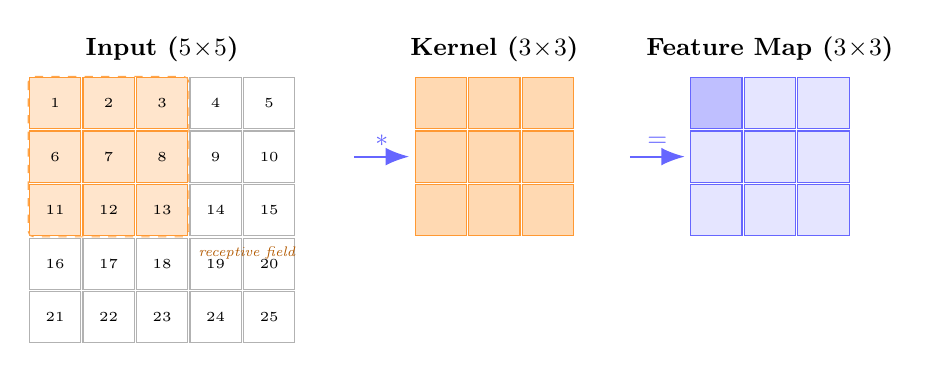
\begin{tikzpicture}[
      cell/.style={rectangle, draw=gray!60, minimum size=0.65cm,
                   inner sep=0, font=\tiny},
      kcell/.style={rectangle, draw=orange!80, fill=orange!20,
                    minimum size=0.65cm, inner sep=0, font=\tiny},
      fcell/.style={rectangle, draw=blue!60, fill=blue!10,
                    minimum size=0.65cm, inner sep=0, font=\tiny},
      lbl/.style={font=\small\bfseries}
    ]
    %% Input 5x5
    \foreach \r in {0,...,4}{
      \foreach \c in {0,...,4}{
        \pgfmathsetmacro{\val}{int(\r*5+\c+1)}
        \ifnum\r<3
          \ifnum\c<3
            \node[kcell] at ({(\c)*0.68},{-(\r)*0.68}) {\val};
          \else
            \node[cell] at ({(\c)*0.68},{-(\r)*0.68}) {\val};
          \fi
        \else
          \node[cell] at ({(\c)*0.68},{-(\r)*0.68}) {\val};
        \fi
      }
    }
    \node[lbl, above=0.3cm] at (1.36, 0.1) {Input ($5\!\times\!5$)};

    %% Arrow
    \draw[-{Latex[length=3mm]}, thick, blue!60]
      (3.8, -0.68) -- node[above, font=\small] {$*$} (4.5, -0.68);

    %% Kernel 3x3
    \foreach \r in {0,...,2}{
      \foreach \c in {0,...,2}{
        \node[kcell, fill=orange!30] at ({4.9+(\c)*0.68},{-(\r)*0.68}) {};
      }
    }
    \node[lbl, above=0.3cm] at (5.58, 0.1) {Kernel ($3\!\times\!3$)};

    %% Arrow
    \draw[-{Latex[length=3mm]}, thick, blue!60]
      (7.3, -0.68) -- node[above, font=\small] {$=$} (8.0, -0.68);

    %% Output 3x3
    \foreach \r in {0,...,2}{
      \foreach \c in {0,...,2}{
        \node[fcell] at ({8.4+(\c)*0.68},{-(\r)*0.68}) {};
      }
    }
    \node[fcell, fill=blue!25] at ({8.4},{0}) {};
    \node[lbl, above=0.3cm] at (9.08, 0.1) {Feature Map ($3\!\times\!3$)};

    %% Annotation
    \draw[dashed, orange!70, rounded corners=2pt]
      (-0.34, 0.34) rectangle (1.7, -1.7)
      node[below right, font=\tiny\itshape, text=orange!70!black]
      {receptive field};
  \end{tikzpicture}
  \caption{Convolution of a $5\!\times\!5$ input with a $3\!\times\!3$ kernel
           produces a $3\!\times\!3$ feature map.  The orange highlighted
           region is the \emph{receptive field} --- the local patch used to
           compute the top-left output value.  The kernel slides across all
           valid positions.}
  \label{fig:convolution}
\end{figure}

\subsection{Kernels and Feature Maps}
\label{sec:cnn_intro:kernels}

The CNN slide (V08, timestamp 1:01:01) stated the following key points
verbatim:

\begin{enumerate}
  \item CNNs are designed for processing 2D data such as images.
  \item CNNs use the \emph{convolution operation} in place of matrix
        multiplication in at least one of their layers.
  \item The output of convolving an input with a kernel is called a
        \textbf{feature map}.
  \item The goal is to \emph{learn} appropriate values for the kernel using a
        suitable learning algorithm (backpropagation).
  \item Each kernel will represent a meaningful pattern once learning is
        complete (e.g., edge detectors, texture filters).
\end{enumerate}

\begin{definition}[Feature Map]
  \label{def:feature_map}
  A \emph{feature map} is the output tensor produced by applying a single
  learned kernel to the input.  If $C_{\text{in}}$ input channels are each
  convolved with the same kernel and the results summed, one feature map
  of size $(H - k + 1) \times (W - k + 1)$ is produced.  Using $C_{\text{out}}$
  distinct kernels produces $C_{\text{out}}$ feature maps stacked as a
  3-D output tensor.
\end{definition}

\begin{remark}
  \label{rem:weight_sharing}
  The key computational advantage of convolution is \emph{weight sharing}:
  the same $k \times k$ kernel is applied at \emph{every} position of the
  input.  This drastically reduces the number of learnable parameters
  compared to a fully-connected layer and makes the model
  \emph{translation-equivariant} (detecting a pattern anywhere in the image
  uses the same kernel weights).
\end{remark}

\subsection{CNN Architecture Overview}
\label{sec:cnn_intro:arch}

A complete CNN consists of two functional stages:

\begin{enumerate}
  \item \textbf{Feature extraction backbone}: stacked convolutional layers
        (each followed by an activation and optionally a pooling layer) that
        progressively transform the raw pixel grid into abstract
        feature representations.
  \item \textbf{Classifier head}: one or more fully-connected layers that
        map the extracted features to class scores.
\end{enumerate}

\cref{fig:cnn_pipeline} provides a schematic of the full pipeline.

\begin{figure}[htbp]
  \centering
  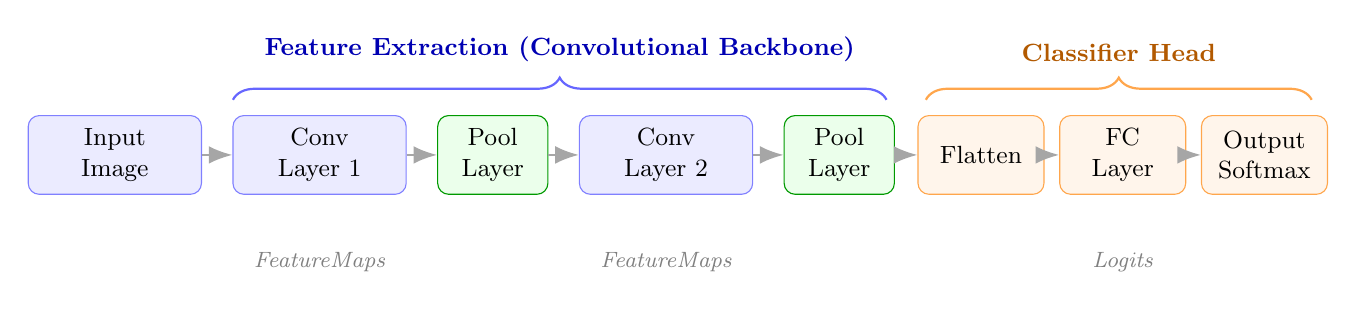
\begin{tikzpicture}[
      block/.style={rectangle, draw=blue!50, fill=blue!8,
                    rounded corners=4pt, minimum width=2.2cm,
                    minimum height=1.0cm, align=center, font=\small},
      pool/.style={rectangle, draw=green!60!black, fill=green!8,
                   rounded corners=4pt, minimum width=1.4cm,
                   minimum height=1.0cm, align=center, font=\small},
      fc/.style={rectangle, draw=orange!70, fill=orange!8,
                 rounded corners=4pt, minimum width=1.6cm,
                 minimum height=1.0cm, align=center, font=\small},
      arr/.style={-{Latex[length=3mm]}, gray!70, line width=0.8pt},
      lbl/.style={font=\footnotesize\itshape, text=gray}
    ]
    \node[block] (inp)  at (0,0)    {Input\\Image};
    \node[block] (c1)   at (2.6,0)  {Conv\\Layer 1};
    \node[pool]  (p1)   at (4.8,0)  {Pool\\Layer};
    \node[block] (c2)   at (7.0,0)  {Conv\\Layer 2};
    \node[pool]  (p2)   at (9.2,0)  {Pool\\Layer};
    \node[fc]    (flat) at (11.0,0) {Flatten};
    \node[fc]    (fc1)  at (12.8,0) {FC\\Layer};
    \node[fc]    (out)  at (14.6,0) {Output\\Softmax};

    \foreach \a/\b in {inp/c1, c1/p1, p1/c2, c2/p2, p2/flat, flat/fc1, fc1/out}{
      \draw[arr] (\a) -- (\b);
    }

    \node[lbl, below=0.6cm of c1] {Feature\\Maps};
    \node[lbl, below=0.6cm of c2] {Feature\\Maps};
    \node[lbl, below=0.6cm of fc1] {Logits};

    \draw[decorate, decoration={brace,amplitude=8pt},
          blue!60, thick]
      (1.5, 0.7) -- (9.8, 0.7)
      node[midway, above=10pt, font=\small\bfseries, text=blue!70!black]
      {Feature Extraction (Convolutional Backbone)};

    \draw[decorate, decoration={brace,amplitude=8pt},
          orange!70, thick]
      (10.3, 0.7) -- (15.2, 0.7)
      node[midway, above=10pt, font=\small\bfseries, text=orange!70!black]
      {Classifier Head};
  \end{tikzpicture}
  \caption{Schematic of a typical CNN pipeline: convolutional and pooling
           layers extract hierarchical spatial features; fully-connected
           layers perform the final classification.}
  \label{fig:cnn_pipeline}
\end{figure}

% ============================================================
\section{Student Q\&A: Key Clarifications}
\label{sec:qa}
% ============================================================

The session included an extended Q\&A period covering important subtleties.
The most significant exchanges are summarised below.

\subsection{Dropout during Backpropagation}
\label{sec:qa:dropout_backprop}

\textbf{Question}: When neurons are dropped during the forward pass, are
their weights also updated during backpropagation?

\textbf{Answer} (paraphrased): For a given mini-batch, only the
\emph{active} sub-network (the network with dropped neurons removed) is
used for both the forward pass and the backward pass.  The weights connected
to dropped neurons receive no gradient for that mini-batch.  However, since
dropping is \emph{random}, different weights are updated at different
mini-batches, ensuring all weights accumulate gradient over the full
training run.

\subsection{ReLU vs.\ Dropout}
\label{sec:qa:relu_vs_dropout}

\textbf{Question}: ReLU also sets negative activations to zero --- is it
not similar to dropout?

\textbf{Answer}: Both zero out activations, but in fundamentally different
ways:

\begin{itemize}
  \item \textbf{ReLU} zeros activations deterministically based on the
        \emph{sign} of the pre-activation value.  There is no guarantee
        about \emph{how many} neurons will be suppressed.
  \item \textbf{Dropout} zeros activations \emph{randomly} with a fixed
        probability $p$.  This guarantees that exactly $p \times n$ neurons
        are zeroed (on average), regardless of activation values, forcing the
        network to build robust, distributed representations.
\end{itemize}

\subsection{Effect of Dropout on Convergence}
\label{sec:qa:convergence}

\textbf{Question}: Does dropout slow down convergence?

\textbf{Answer}: There are two competing effects:

\begin{enumerate}
  \item \textbf{Fewer parameters per step}: dropping 30\,\% of neurons means
        30\,\% fewer weight updates per mini-batch, which \emph{reduces} the
        computation per step and may slightly accelerate wall-clock training.
  \item \textbf{Noisier gradient estimates}: the effective network changes
        every batch, introducing variance into the gradient signal, which
        may require more epochs to converge.
\end{enumerate}

Net effect: dropout can slow convergence slightly but produces a model that
\emph{generalises better}, which is the primary objective.

% ============================================================
\section{Summary and Conclusion}
\label{sec:summary}
% ============================================================

\subsection{Session Recap}
\label{sec:summary:recap}

Session 12 covered three main threads:

\begin{enumerate}
  \item \textbf{Diagnosing overfitting}: A 10\,\% train/test accuracy gap
        (98\,\% vs.\ 88\,\%) in the Version 2 ANN was identified as
        evidence of overfitting and the target for regularisation.

  \item \textbf{Three regularisation strategies}:
    \begin{itemize}
      \item \textbf{$\Ltwo$ weight decay} adds a quadratic penalty
            $\lambda\sum_i w_i^2$ to the loss, discouraging large weights and
            simplifying the decision boundary.
      \item \textbf{Batch Normalisation} normalises pre-activation values
            within each mini-batch, stabilising training and reducing internal
            covariate shift.  Placement: \emph{after Linear, before ReLU}.
      \item \textbf{Dropout} randomly zeroes $p$-fraction of neurons during
            training, acting as an implicit ensemble and preventing
            co-adaptation.  Placement: \emph{after ReLU}.
    \end{itemize}

  \item \textbf{CNN Introduction}: Prof.\ Prasanna motivated CNNs from the
        failure of flattening to preserve spatial structure, reviewed the
        ImageNet breakthrough, and formally defined the convolution operation,
        kernels, and feature maps as foundations for the upcoming hands-on
        sessions.
\end{enumerate}

\subsection{Mathematical Summary}
\label{sec:summary:math}

\begin{align}
  \mathcal{L}_{\text{total}}
    &= \mathcal{L}_{\text{data}} + \lambda \sum_i w_i^2
    & &(\Ltwo\text{ regularisation}) \label{eq:summary_l2} \\[4pt]
  \hat{z}_i
    &= \frac{z_i - \mu_\mathcal{B}}{\sqrt{\sigma^2_\mathcal{B}+\varepsilon}},
      \quad y_i = \gamma\hat{z}_i + \beta
    & &(\text{Batch Normalisation}) \label{eq:summary_bn} \\[4pt]
  \tilde{h}_i
    &= m_i \cdot h_i, \quad m_i \sim \mathrm{Bernoulli}(1-p)
    & &(\text{Dropout}) \label{eq:summary_dropout} \\[4pt]
  S(i,j)
    &= \sum_{m,n} X(i+m,j+n)\cdot K(m,n)
    & &(\text{2-D Convolution}) \label{eq:summary_conv}
\end{align}

\subsection{Looking Ahead}
\label{sec:summary:ahead}

Session 13 will dive into the full CNN theory: convolutional layers with
multiple input/output channels, padding and stride, pooling layers, and the
complete LeNet-style architecture applied to image classification.  The
Fashion-MNIST dataset will be revisited using a CNN to demonstrate the
accuracy gains possible over the ANN baseline.

\begin{keyinsight}
  The transition from ANN to CNN is not merely about adding convolution layers
  --- it represents a shift in \emph{inductive bias}.  By assuming local
  connectivity and weight sharing, CNNs encode the prior belief that
  \emph{spatial proximity matters}, which is a highly effective prior for
  image, audio, and time-series data.
\end{keyinsight}

% ============================================================
%% References (manual, as no .bib file)
% ============================================================
\begin{thebibliography}{9}

\bibitem{xiao2017fashionmnist}
H.\ Xiao, K.\ Rasul, and R.\ Vollgraf,
``Fashion-MNIST: a novel image dataset for benchmarking machine learning
  algorithms,''
\textit{arXiv preprint arXiv:1708.07747}, 2017.

\bibitem{ioffe2015batchnorm}
S.\ Ioffe and C.\ Szegedy,
``Batch normalization: Accelerating deep network training by reducing
  internal covariate shift,''
in \textit{Proceedings of ICML}, 2015, pp.\ 448--456.

\bibitem{srivastava2014dropout}
N.\ Srivastava, G.\ Hinton, A.\ Krizhevsky, I.\ Sutskever, and R.\ Salakhutdinov,
``Dropout: A simple way to prevent neural networks from overfitting,''
\textit{Journal of Machine Learning Research}, vol.\ 15, pp.\ 1929--1958, 2014.

\bibitem{lecun1989cnn}
Y.\ LeCun, B.\ Boser, J.\ Denker, D.\ Henderson, R.\ Howard, W.\ Hubbard,
and L.\ Jackel,
``Backpropagation applied to handwritten zip code recognition,''
\textit{Neural Computation}, vol.\ 1, no.\ 4, pp.\ 541--551, 1989.

\bibitem{krizhevsky2012alexnet}
A.\ Krizhevsky, I.\ Sutskever, and G.\ E.\ Hinton,
``ImageNet classification with deep convolutional neural networks,''
in \textit{Advances in Neural Information Processing Systems (NeurIPS)},
2012, pp.\ 1097--1105.

\end{thebibliography}

\clearpage

\end{document}
